%%%%%%%%%%%%%%%%%%%%%%%%%%%%%%%%%%%%%%%%%%%%%%%%%%%%%%%%%%%%%%%%%%%%%%%%%%%%%%%%
%2345678901234567890123456789012345678901234567890123456789012345678901234567890
%        1         2         3         4         5         6         7         8


\documentclass[letterpaper, 10 pt, conference]{ieeeconf}  % Comment this line out
                                                          % if you need a4paper
%\documentclass[a4paper, 10pt, conference]{ieeeconf}      % Use this line for a4
                                                          % paper

\IEEEoverridecommandlockouts                              % This command is only
                                                          % needed if you want to
                                                          % use theplp \thanks command
\overrideIEEEmargins
% See the \addtolength command later in the file to balance the column lengths
% on the last page of the document



% The following packages can be found on http:\\www.ctan.org
\usepackage{graphics} % for pdf, bitmapped graphics files
\usepackage{epsfig} % for postscript graphics files
\usepackage{mathptmx} % assumes new font selection scheme installed
\usepackage{times} % assumes new font selection scheme installed
\usepackage{amsmath} % assumes amsmath package installed
\usepackage{amssymb}  % assumes amsmath package installed
\usepackage{mathtools}
\usepackage[noadjust]{cite}
\usepackage{dblfloatfix}
\usepackage{color}
\usepackage{booktabs,tabularx}
\usepackage{optidef}

\renewcommand{\thefigure}{\arabic{figure}}

\title{\LARGE \bf
Development of Fabric Soft-Poly Limb for Mobile Manipulation of Daily Living Tasks  
}

%\author{ \parbox{3 in}{\centering Huibert Kwakernaak*
%         \thanks{*Use the $\backslash$thanks command to put information here}\\
%         Faculty of Electrical Engineering, Mathematics and Computer Science\\
%         University of Twente\\
%         7500 AE Enschede, The Netherlands\\
%         {\tt\small h.kwakernaak@autsubmit.com}}
%         \hspace*{ 0.5 in}
%         \parbox{3 in}{ \centering Pradeep Misra**
%         \thanks{**The footnote marks may be inserted manually}\\
%        Department of Electrical Engineering \\
%         Wright State University\\\textbf
%         Dayton, OH 45435, USA\\
%         {\tt\small pmisra@cs.wright.edu}}
%}

\author{Pham H. Nguyen, \textit{Student Member, IEEE}, Imran I. B. Mohd, Curtis Sparks, Francisco L. Arellano,\\ and Panagiotis Polygerinos$^{*}$, \textit{Member, IEEE}% <-this % stops a space
%\thanks{*Equally Contributing 1st Authors}% <-this % stops a space
\thanks{$*$ Corresponding Author}% <-this % stops a space
\thanks{Pham H. Nguyen, Curtis Sparks, and Panagiotis Polygerinos are with the Polytechnic School, Ira A. Fulton Schools of Engineering, Arizona State University, Mesa, AZ 85212, USA.} 
\thanks{Imran I. B. Mohd The School for Engineering of Matter, Transport and Energy, Ira A. Fulton Schools of Engineering, Arizona State University, Tempe, AZ 85281, USA.}
\thanks{Francisco L. Arellano The School of Biological Health Systems Engineering, Ira A. Fulton Schools of Engineering, Arizona State University, Tempe, AZ 85281, USA.
        {\tt\small nhpham2@asu.edu, imohd@asu.edu, cmspark1@asu.edu, flopezar@asu.edu, polygerinos@asu.edu}}%
}



\begin{document}



\maketitle
\thispagestyle{empty}
\pagestyle{empty}


%%%%%%%%%%%%%%%%%%%%%%%%%%%%%%%%%%%%%%%%%%%%%%%%%%%%%%%%%%%%%%%%%%%%%%%%%%%%%%%%
\begin{abstract}

This paper presents the novel design and development of a highly articulated, continuum, wearable, fabric-based Soft Poly-Limb (fSPL) that acts as an additional limb to provide compliant and safe mobile manipulation assistance to users with upper extremity impairments. In this work, a set of systematic design rules is presented for the creation of highly compliant soft robotic limbs through an understanding of their component’s behavior as a function of input pressure. These design rules are obtained by investigating a range of geometrical parameters of the f3CBAs through computational finite-element method (FEM) models focusing on the fSPL's articulation capabilities and payload capacity in 3D space.  The motion and payload evaluation of the fSPL and its components is performed through experimental validation of the FEM models and preliminary evaluation of its capability to safely operate and interact with the user with spatial mobility tests and pick-and-place experiments while attached to a soft-waist belt that can comfortably store the fSPL when not in use.

\end{abstract}

%%%%%%%%%%%%%%%%%%%%%%%%%%%%%%%%%%%%%%%%%%%%%%%%%%%%%%%%%%%%%%%%%%%%%%%%%%%%%%%%
\section{INTRODUCTION}

Cervical Spondylotic Myelopathy (CSM) is a degenerative condition that is caused by general wear and tear or injury to the cervical region of the spinal cord, affecting limb functions and limiting independence, affecting a spectrum of patients across different age groups \cite{lubelski2016}. CSM can cause upper limb impairment characterized by symptoms such as muscle weakness, numbness, and loss of fine motor control. As a result, individuals with CSM syndrome typically experience difficulty performing motor tasks, such as picking up a cup and other activities of daily living (ADLs). This population could benefit from a soft wearable collaborative robotic device, such as the fabric-based, Soft-Poly Limb (fSPL) presented in this work.

\begin{figure}[t!]
\centering
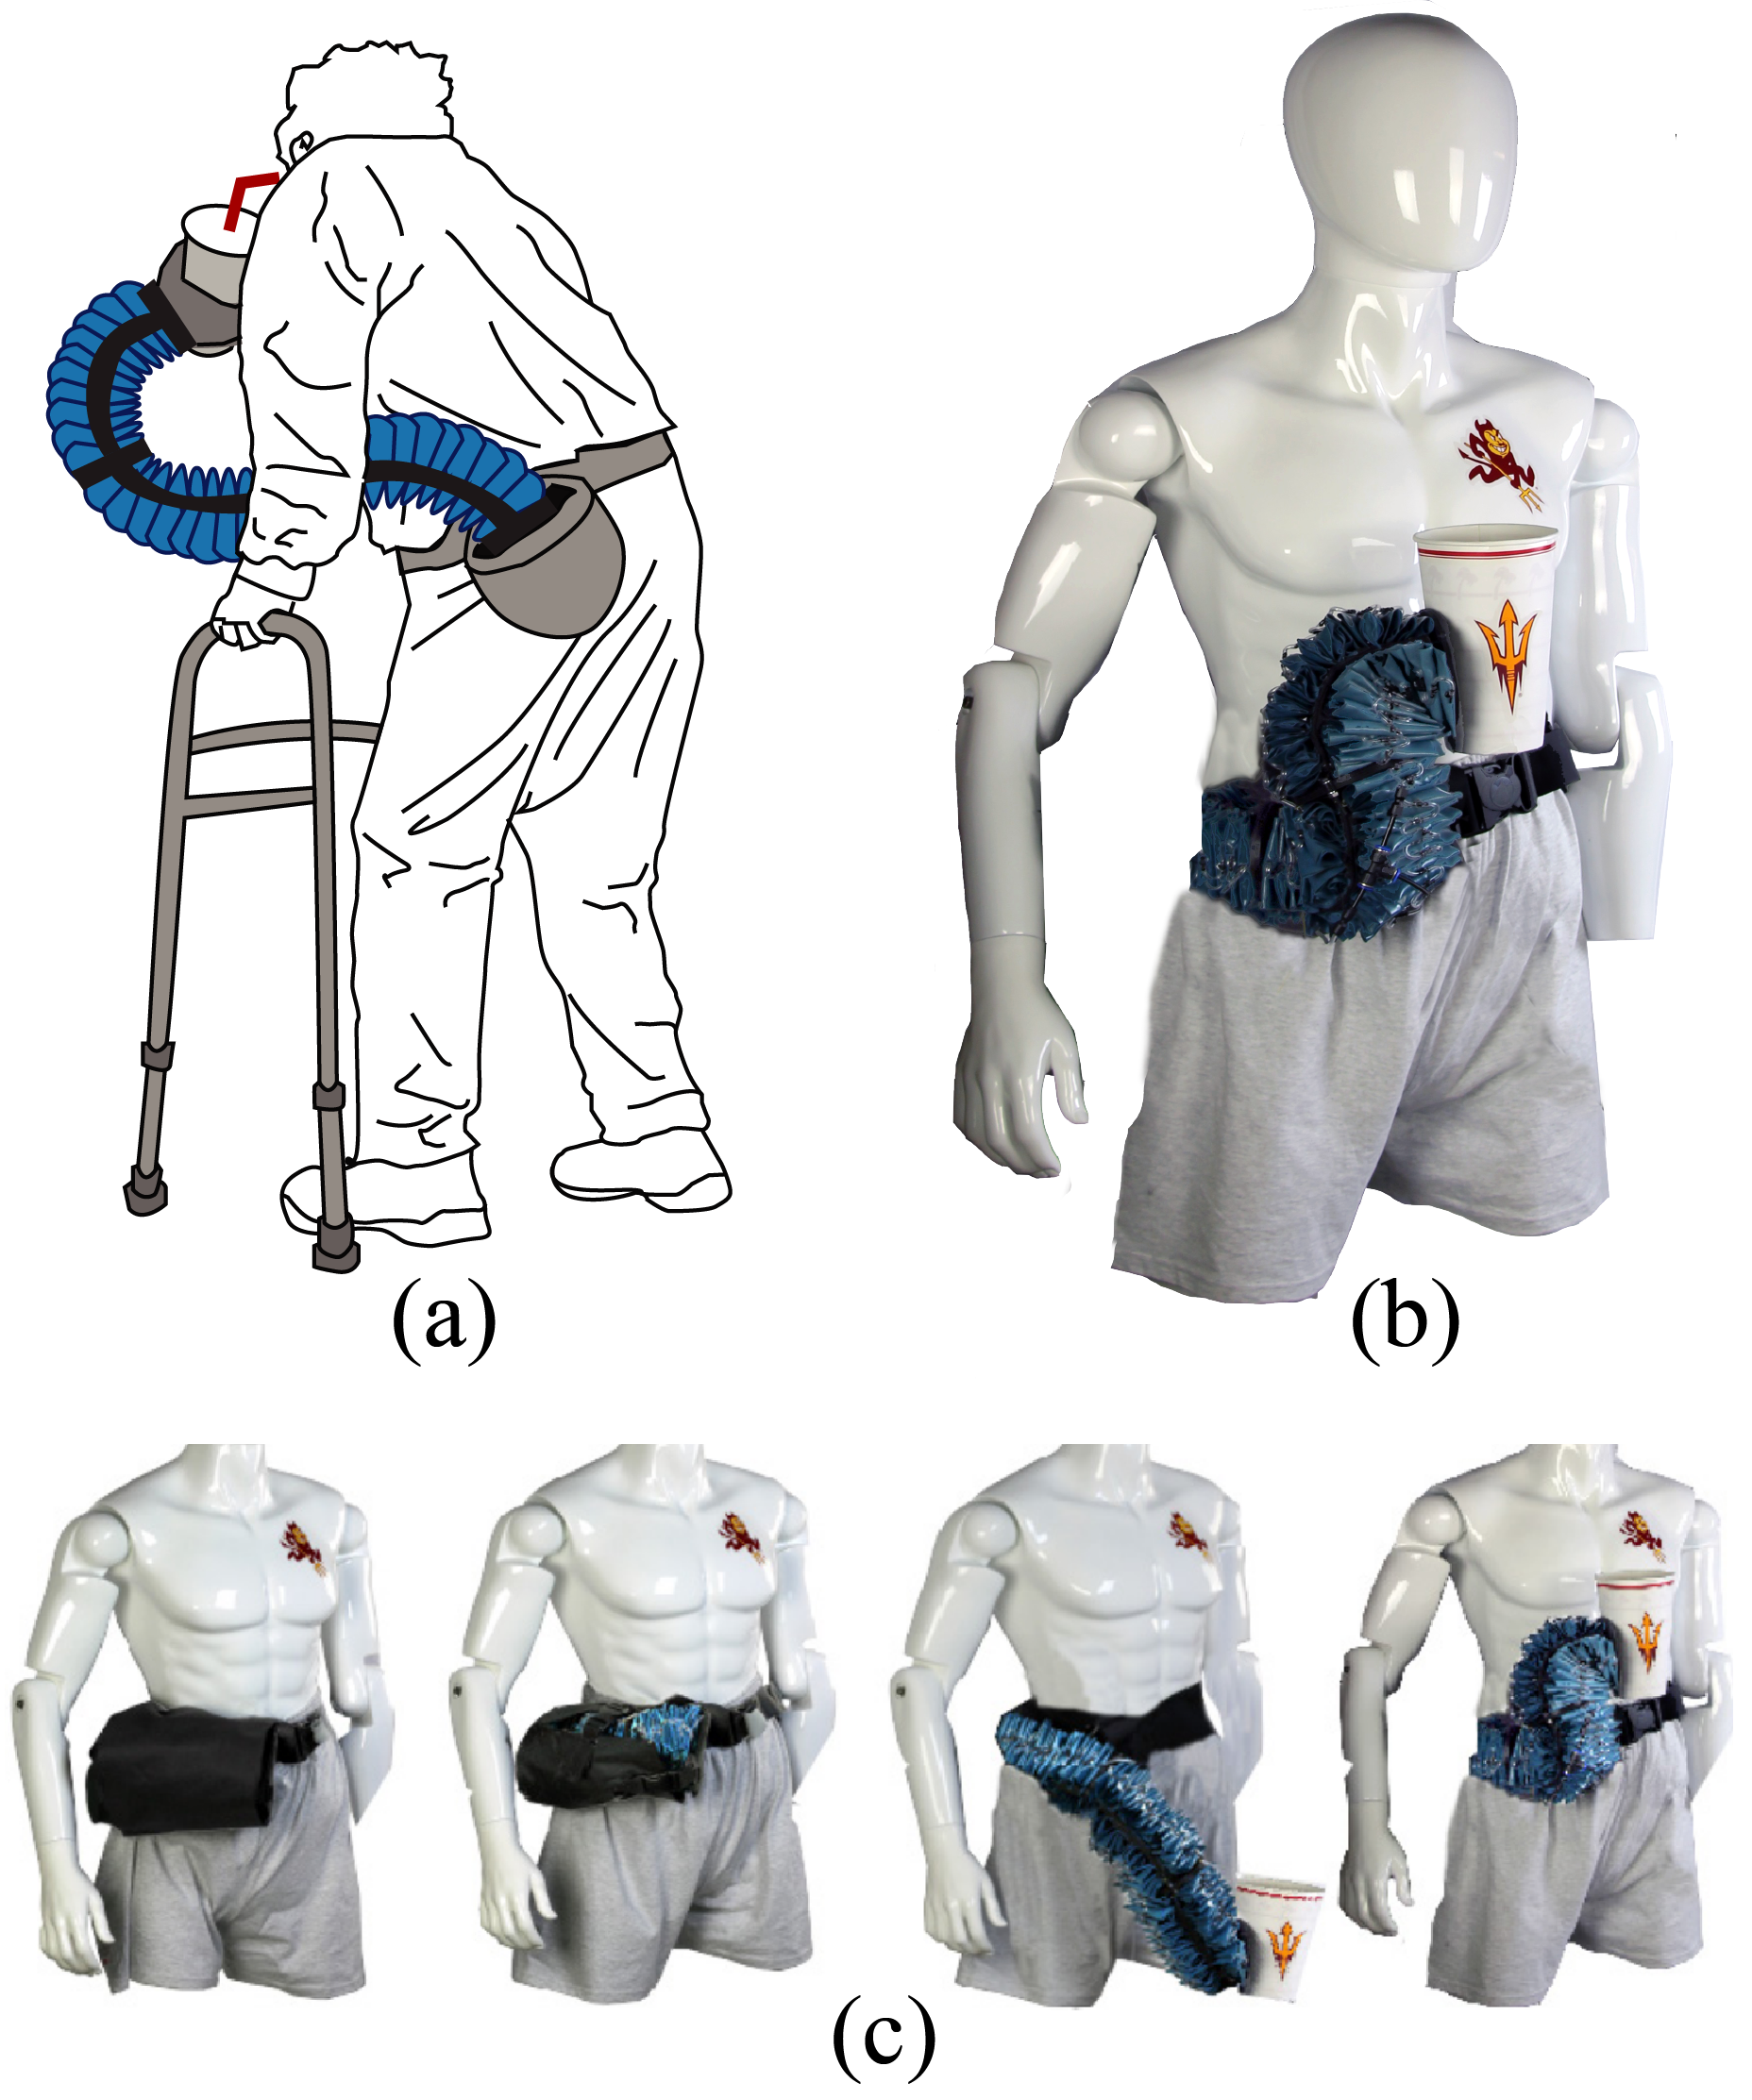
\includegraphics[width=0.45\textwidth]{Figures/fig1_new}
\caption{ (a) Illustrated concept of the fabric-based Soft Poly Limb (fSPL). (b) The prototype fSPL mounted on a lightweight waist-belt system is a soft, lightweight, wearable robot that is designed to assist users with assisted daily living (ADL) tasks. (c) Left-to-right: the limb is collapsed and stored in a pouch and then deployed to assist with daily living tasks, such as picking up a drinking cup.}
\label{fig:fig1}
\vspace{-1.5em}
\end{figure}

Wearable robotics manipulators are devices that can be worn to provide an additional appendage to assist and support the user to perform tasks. These devices do not kinematically have to match the human body's anatomy, like exoskeletons \cite{gopura2011} or prosthetic devices \cite{bogue2009}. Therefore, they do not require extra consideration in terms of alignment with biological joints. Recent examples of different wearable collaborative robotic devices include robotic legs \cite{kurek2017,parietti2015}, arms \cite{parietti2014,saraiji2018,vatsal2017}, fingers \cite{hussain2017b,wu2015,tiziani2017}, ranging from the industrial \cite{parietti2014} and medical settings \cite{tiziani2017}. 

The recent rise of wearable robotic manipulators have brought up questions of user controllability. The possibility of controlling an extra limb has been previously investigated and it is known that the human central nervous system (CNS) is found to be capable of learning to control additional limbs \cite{guterstam2011,tsakiris2010}. The controllability of robotic limbs has been explored in preliminary research, utilizing biological signals from the torso muscles \cite{parietti2017}, foot \cite{sasaki2017}, elbow \cite{wu2015}, and the forehead frontalis muscles \cite{salvietti2017}.

Wearable manipulators currently face limitations that comes with their rigid designs, like their weight, bulk, and the interaction between rigid elements and the human body \cite{delAma2012}. These challenges leads to questions related to safe interaction with the users and could possibly limit adoption of the technology. Soft robotics has emerged as one of the solutions to tackle the aforementioned challenges. The nature of intrinsically soft devices (ISDs) lead to robot designs that are lightweight, low-cost, has a high power-to-weight ratio, and is safe for human-robot interaction but are also highly adaptable and robust to the external environment \cite{polygerinos2016}. This compliant nature promotes psychological acceptance of such soft wearable devices because they can conform to the user's body without injuring them. The recent influx of soft robots have led to the introduction a variety of soft continuum manipulators made of a variety of soft actuators. The categories of soft continuum manipulators is subdivided based on the actuators that constitute them, including cable-driven \cite{mcMahan2005,calisti2011}, pneumatic artificial muscles (PAMs) \cite{walker2005,godage2016,yasmin2017,giannaccini2017}, elastomeric \cite{cianchetti2013,marchese2015,robertson2017,gong2018}, origami \cite{santoso2017}, and inflatable-fabric \cite{sanan2013,hawkes2017,ohta2017,best2016,liang2018,takeichi2017,kim2018,liang2017c} based manipulators. 

The fusion of soft robotics and wearable manipulators has created a new category of robotics which we call, Soft Poly-Limbs (SPLs). Limited research has started to emerge in this category, Tiziani et al. \cite{tiziani2017} has introduced a soft poly-finger device to help patients with grasping, Liang et al. \cite{liang2017c} have suggested a fabric-based soft poly-arm device, with a single degree-of-freedom, that would eventually be integrated as a wearable robot but have not evaluated the device for this use case yet, and finally we have introduced a safe, elastomeric SPL device \textbf{cite[]} with nine degree-of-freedom, and is capable of lifting weights horizontally up to 1.4$x$ its own body weight and wrap around objects to lift approximately 4.07$x$ its own weight. 

In this paper, we have designed a novel, highly-articulated, high-power-to-weight ratio, fabric-based, upper-limb SPL capable of assisting users with ADL tasks, as seen in Fig. 1. We present the components that make up the fabric-based SPL, including: a) the novel design of the fabric-based, 3-DOF, three-chambered bending actuators (f3CBAs) and b) the complete continuum, fabric-based SPL (fSPL) created by the combination of multiple f3CBAs. We provide a material study of various fabric material tested to achieve the current design of the fabric-based SPL (fSPL). We further investigate the mechanical behavior of the limb and its components by using a varying set of design parameters to optimize the payload capacity of the fSPL by using computational finite element method (FEM) models that are also validated experimentally. We also address the possible concerns adopters would have when using such a device, in the ability to don and doff the device, function, and capabilities. Finally, through experimentation we showcase the potential of the novel fSPL to work safely around a user, carry high-payload, and assisting the user with ADLs tasks. 


\section{fSPL Functional Requirements and Design}

\begin{table}[t!]
\caption{Specifications for a fabric-based Soft-Poly Limb (fSPL) Characteristics} 
\label{tab:spec_table}
	\begin{tabularx}{0.48\textwidth}{*2l}    \toprule\toprule
	\textbf{\emph{Characteristics}} & \textbf{\emph{Specifications}} \\\midrule
	Weight of Device    & less than 1.5$kg$  \\ 
	Profile of fSPL & less than 100$mm$ diameter \\ 
	Payload (fully extended)    & Approx. 1$kg$  \\ 
	Payload (whole-body grasp) & 2$x$ the weight of device \\ 
	Max. Reach Length    & Length of male arm (0.59$m$)  \\ 
	Min. Retraction Length & Half of fully stretched SPL \\ 
	Safety    & Easy to don-and-doff \\ 
	 &Does not interfere with\\
     &biological limb's movement\\
	Degrees-of-Freedom (DOF) & At least 9DOF \\ 
	Degrees of Curvature of Each Segment & 180$^{\circ}$ \\\bottomrule
	 \hline
	\end{tabularx}
\end{table}

In order to provide long-term options to CSM patients who have loss/reduced function in their hands and arms, for their day-to-day tasks, we have laid out a soft robotic architecture with versatile specifications summarized in Table \ref{tab:spec_table}. We intend to provide the users with a highly deployable, full-length SPL that interacts safely with the user, and can be compressed to at least half of its original length and stowed away in a small pouch attached to a waist belt, without providing extra bulkiness while still being extremely light weight (under 1.5$kg$). The SPL should be a highly maneuverable continuum manipulator with 9-DOFs, while being compliant and configurable. The system would be able to carry up to approximately 1$kg$ of payload at its end-effector position when fully-extended and parallel to the ground and carry up to twice its body weight by wrapping around the object using the continuum whole-body grasping method. 

In order to achieve the design characteristics as mentioned above, we have designed a fabric-based, full-length, Soft-Poly Limb made up of three modular segments called the fabric-based, 3-chambered bending actuator (f3CBAs), each of which is designed with 3 arrays of bending actuators arranged in an equilateral triangle fashion. The length of the SPL is designed to approximately match the length of an average sized adult male arm, which is approximately 0.59$m$, from the tip of the shoulder to the center of the wrist. Each of the fSPL segments therefore has a length of 0.16$m$. 

Each bending actuator array is comprised of multiple high-strength, heat-sealed, TPU-coated nylon (200D) fabric actuators that are arranged and sewn onto a strain-limited fabric layer. The functionality of the bending actuator arrays have previously been highlighted in our previous work \cite{thalman2018} where thermoplastic polyurethane (TPU) actuators were encased in nylon fabric casings in order to withstand higher pressure of up to 0.3$kPa$. In this paper, a variety of heat-sealable TPU-coated nylon fabric material are explored to create actuators that are robust to external environmental interaction, allows for a single-step fabrication process that saves manufacturing time, and is capable of withstanding pressures up to 0.53$MPa$, thus achieving higher torque generation.

Customization is also a key factor emphasized to allow for improved future adoption of the fSPL. The segments of the fSPL and the actuators in the actuator array are interchangeable and easily replaceable for required maintenance. The fSPL can be compressed to half its full length allowing for ease of carriage. The fSPL is mounted on a comfortable waist belt system that weighs 0.5$kg$ that allows the integrated wearable device to don-doff easily. The end-effector unit is also customizable for the specified task. The fSPL is also capable of utilizing its entire soft body to grasp and carry objects larger in size and weight, something that traditional rigid robotic arms are incapable of achieving. The pneumatic system is currently off-board and controlled by our experimental platform \cite{nguyen2018} to monitor and control the SPL.





% \begin{figure}[t]
% \centering
% 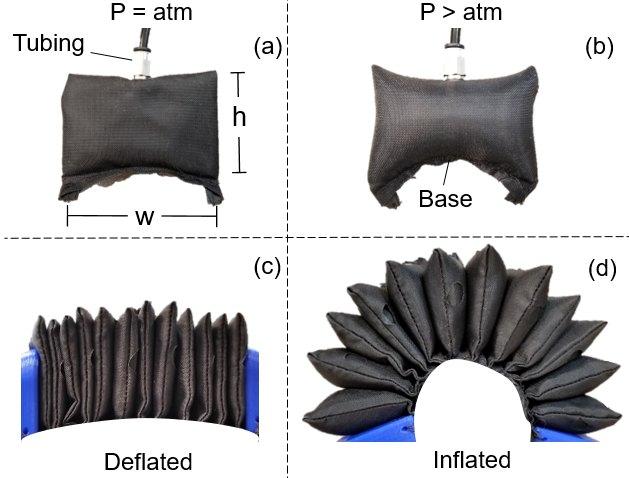
\includegraphics[width=0.4\textwidth]{V1_device.PNG}
% \caption{(a) Deflated soft actuator with labeled dimensions for width, $w$ and height, $h$. (b) Inflated soft actuator. (c) Deflated soft actuator array. (d) Inflated soft actuator array.
% }

% \label{fig:array}
% \end{figure}




% \begin{figure}
% \centering
% 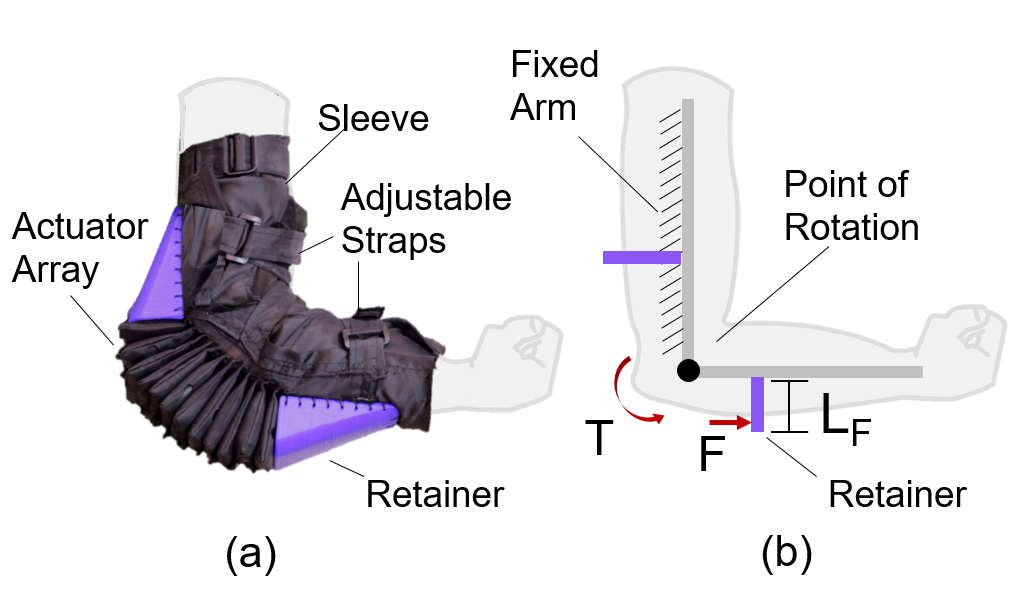
\includegraphics[width=0.45\textwidth]{arm.PNG}
% \caption{Final Design of the soft robotic elbow sleeve (left) and the governing free body diagram (FBD) of the actuator array against the elbow (right)}
% \label{fig:arm}
% \vspace{-1.5em}
% \end{figure}
 
\section{SPl Design and Characterization} 

\subsection{Material Selection and Characterization}
\label{sec:mat_select}


\begin{table}[t!]
\caption{Material Properties of TPU Coated Nylon Fabrics} 
\label{tab:materialproperty_table}
	\begin{tabularx}{0.48\textwidth}{l|c|c|c}   \toprule\toprule
    \centering
    \small
    \setlength\tabcolsep{11pt}
	\textbf{\emph{Material}} & \textbf{\emph{Density (N) }} & \textbf{\emph{Seal Strength}} & \textbf{\emph{Burst }} \\[-1pt]
                             &                              & \textbf{\emph{(kg/m$^3$)}} & \textbf{\emph{Strength}}\\
                             &                              &                            & \textbf{\emph{(MPa)}}\\\midrule
	Rockywoods 200D &840.00 &168.35 & 0.53 \\
    Outdoor Oxford 200D  &757.58 &  183.68 & 0.48\\
    Ripstop 200D &758.62 & 192.19 & 0.30\\
    Seatle Diamond 200D &892.86 & 164.75 & 0.36\\
    DIY Packraft 400D & 982.46& 155.32 & x\\
    DIY Packraft 1000D &1000.00 & 236.17 & x\\
    Taffeta 70D &700.00& 142.13 & x\\\bottomrule 
    \hline
	\end{tabularx}
\end{table}

To design the fSPL with a high payload capacity yet be lightweight and robust to external interaction, a set of TPU-coated nylon fabrics with dernier values ranging from 70D to a 100D, indicating the fiber thickness of the filament used, as seen in Table \ref{tab:materialproperty_table}. To determine the material to be used for the actuator, standardized testing methods for seal strength (ASTM F88/F88M-15), burst strength (ASTM F2054) and tensile properties (ASTM D882) were conducted.

Firstly, the individual bladders need to be able to maintain a tight seal under high stresses in order to remain airtight. The TPU seal strength for each material is tested using the ASTM F88/F88M-15 standard which involves applying axial tensile stress on the seal of the TPU-coated nylon fabrics. The test for each material was conducted 3 times and the average maximum seal strength values were calculated and tabulated as seen in Table \ref{tab:materialproperty_table}. The materials with the highest seal strength were proceeded for further testing. Although the seal strength for the DIY packraft 1000D material was the highest, it was deemed unviable because its incompressibility and density, which would affect the weight and retraction length of the fSPL.  

The chosen materials were tested for their maximum burst strength using ASTM F2054. Three tests were conducted for each material and the average maximum pressure value was recorded in Table \ref{tab:materialproperty_table}. Based on the results, the Rockywoods 200D heat-sealable TPU-nylon fabric (Rockywoods Fabric, Loveland, CO) was chosen for its highest burst strength of 0.53$MPa$.

Finally, the elastic modulus for the selected material is determined using ASTM D882, where axial tensile stress is applied to a fabric piece with measurements of 0.26x0.00254$m$ with a rate of 25$mm/min$ until failure. The calculated Young’s Modulus of Rockywoods 200D is calculated to be 498.9 $MPa$.



\subsection{Geometrical Parameters}

\begin{figure}[b!]
\centering
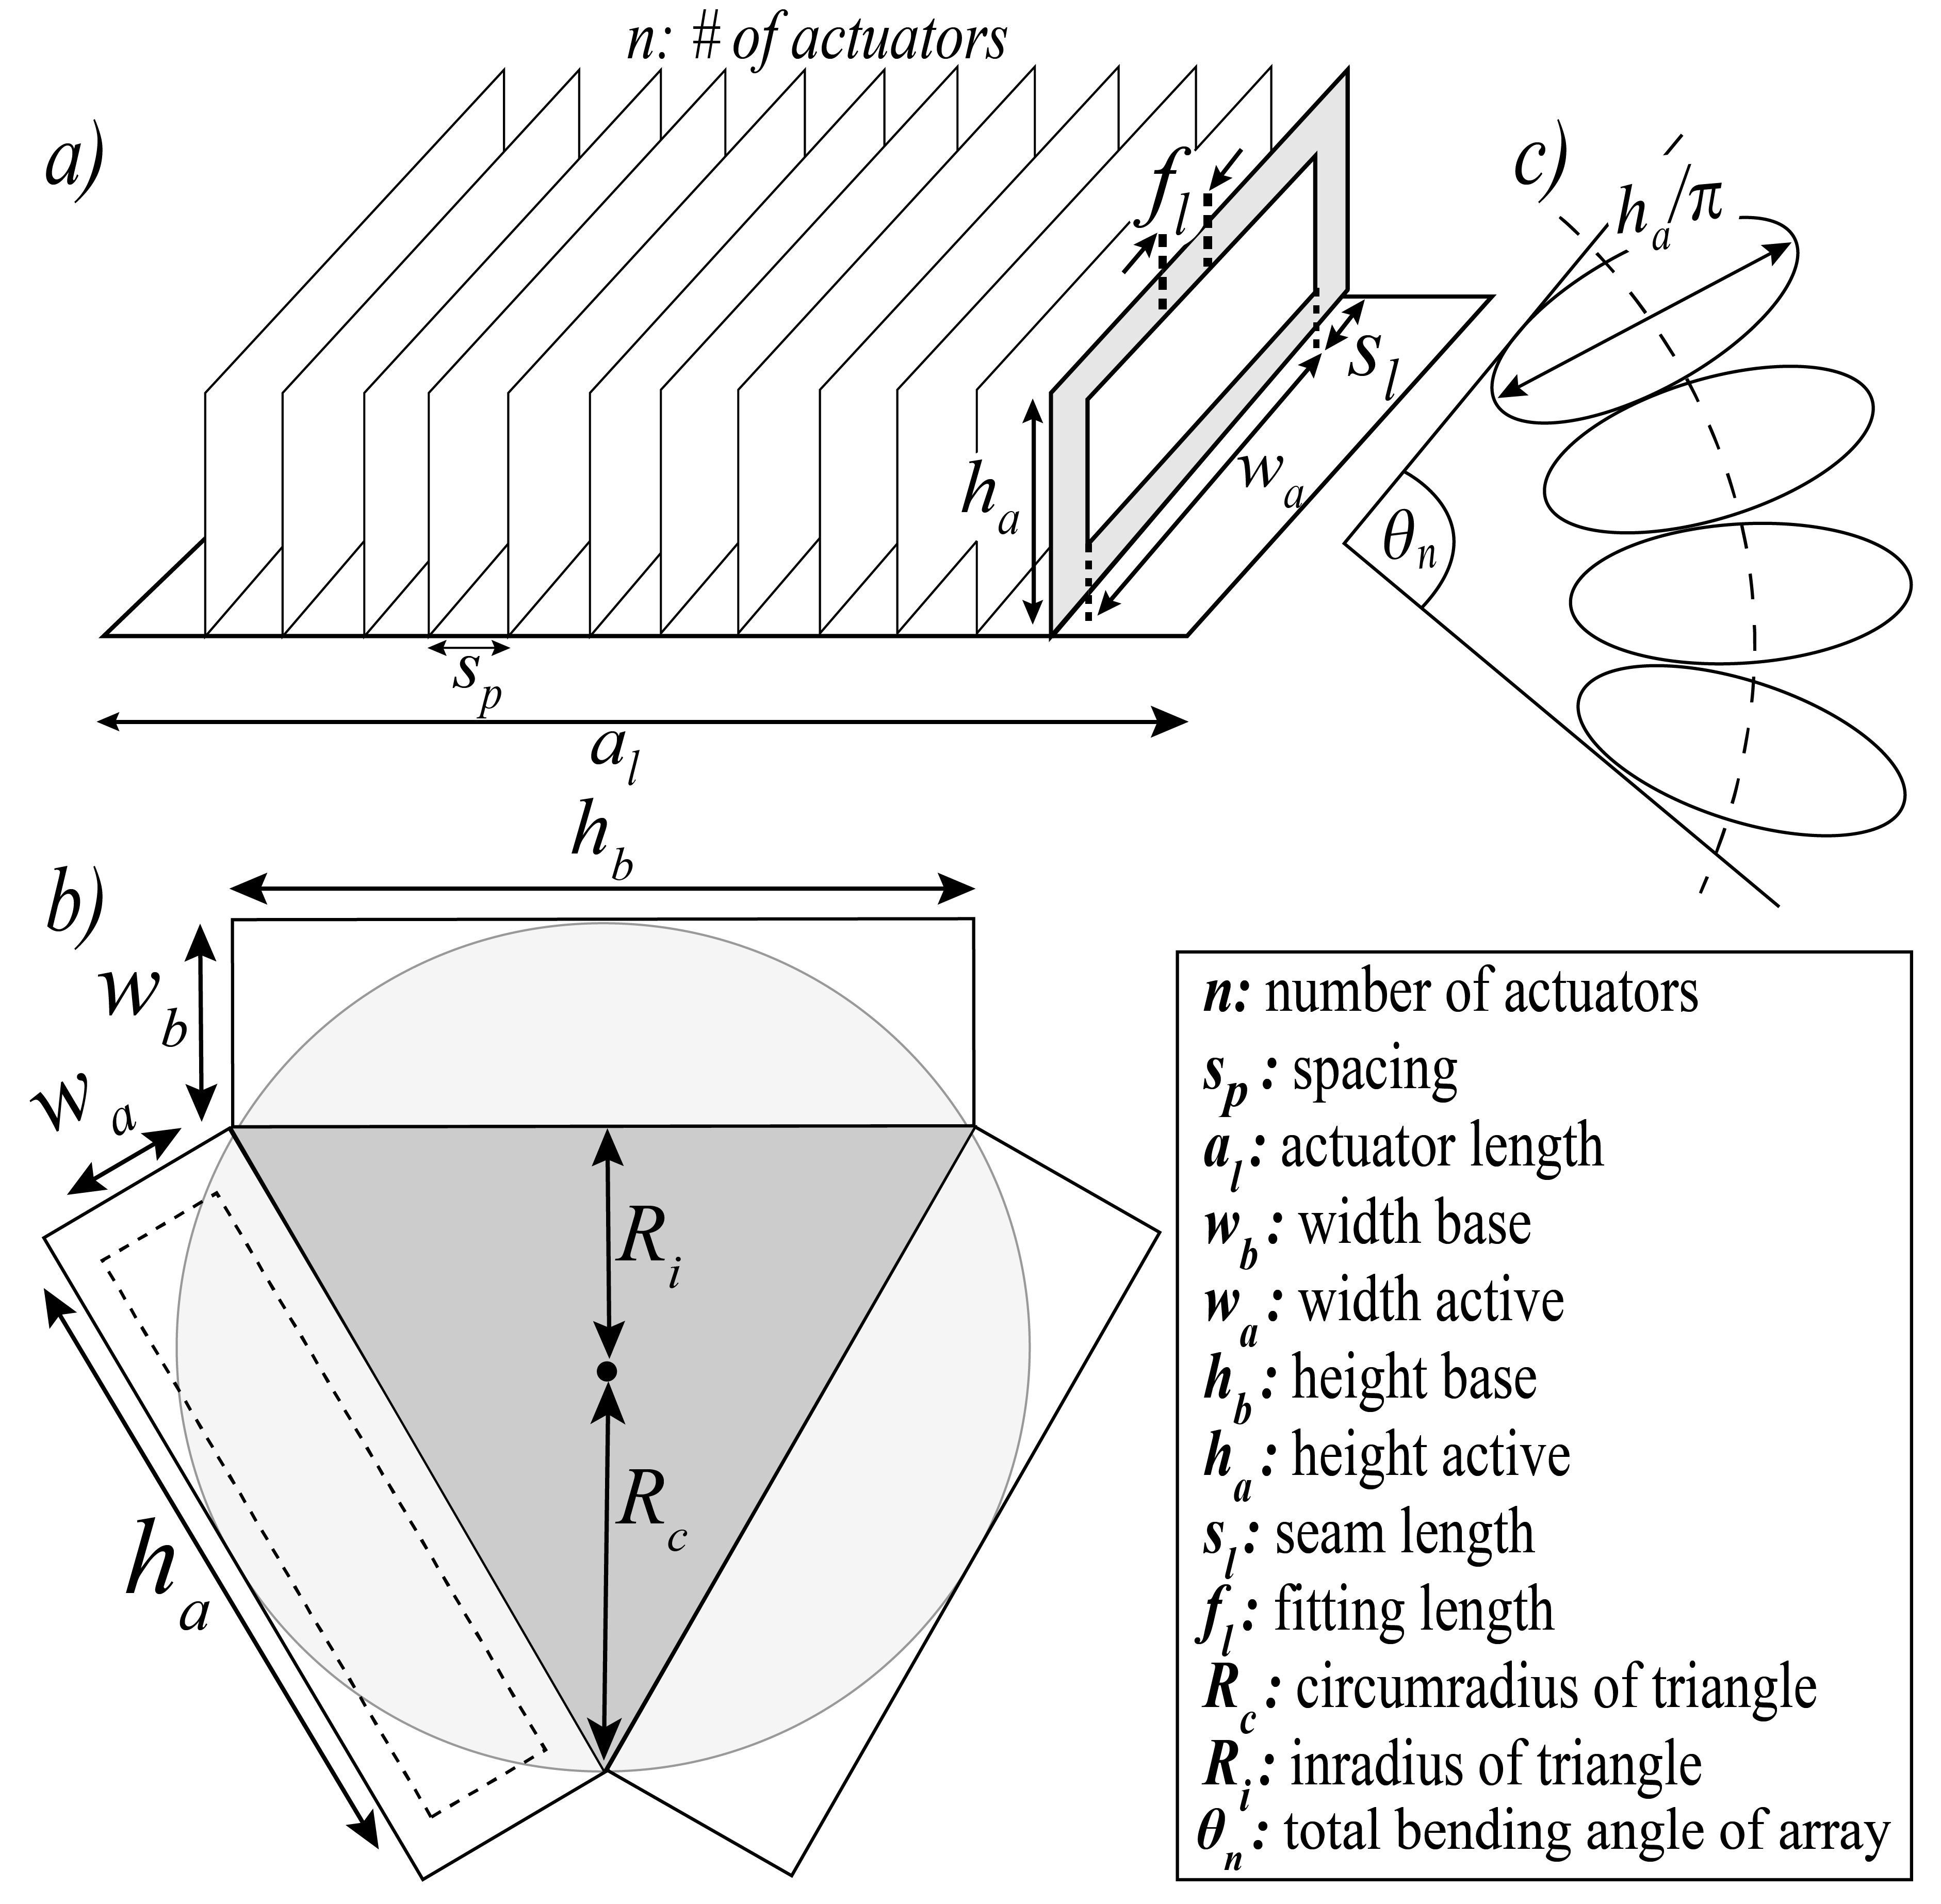
\includegraphics[width=0.5\textwidth]{Figures/geom_param_v5}
\caption{Geometrical Parameters of fSPL. a)Isometric view of bladder actuator array. b) Bottom view of f3CBA. c) Side view of bending bladder actuator array.}
\label{fig:geom_param}
\vspace{-1.5em}
\end{figure}


\begin{figure}[t!]
\centering
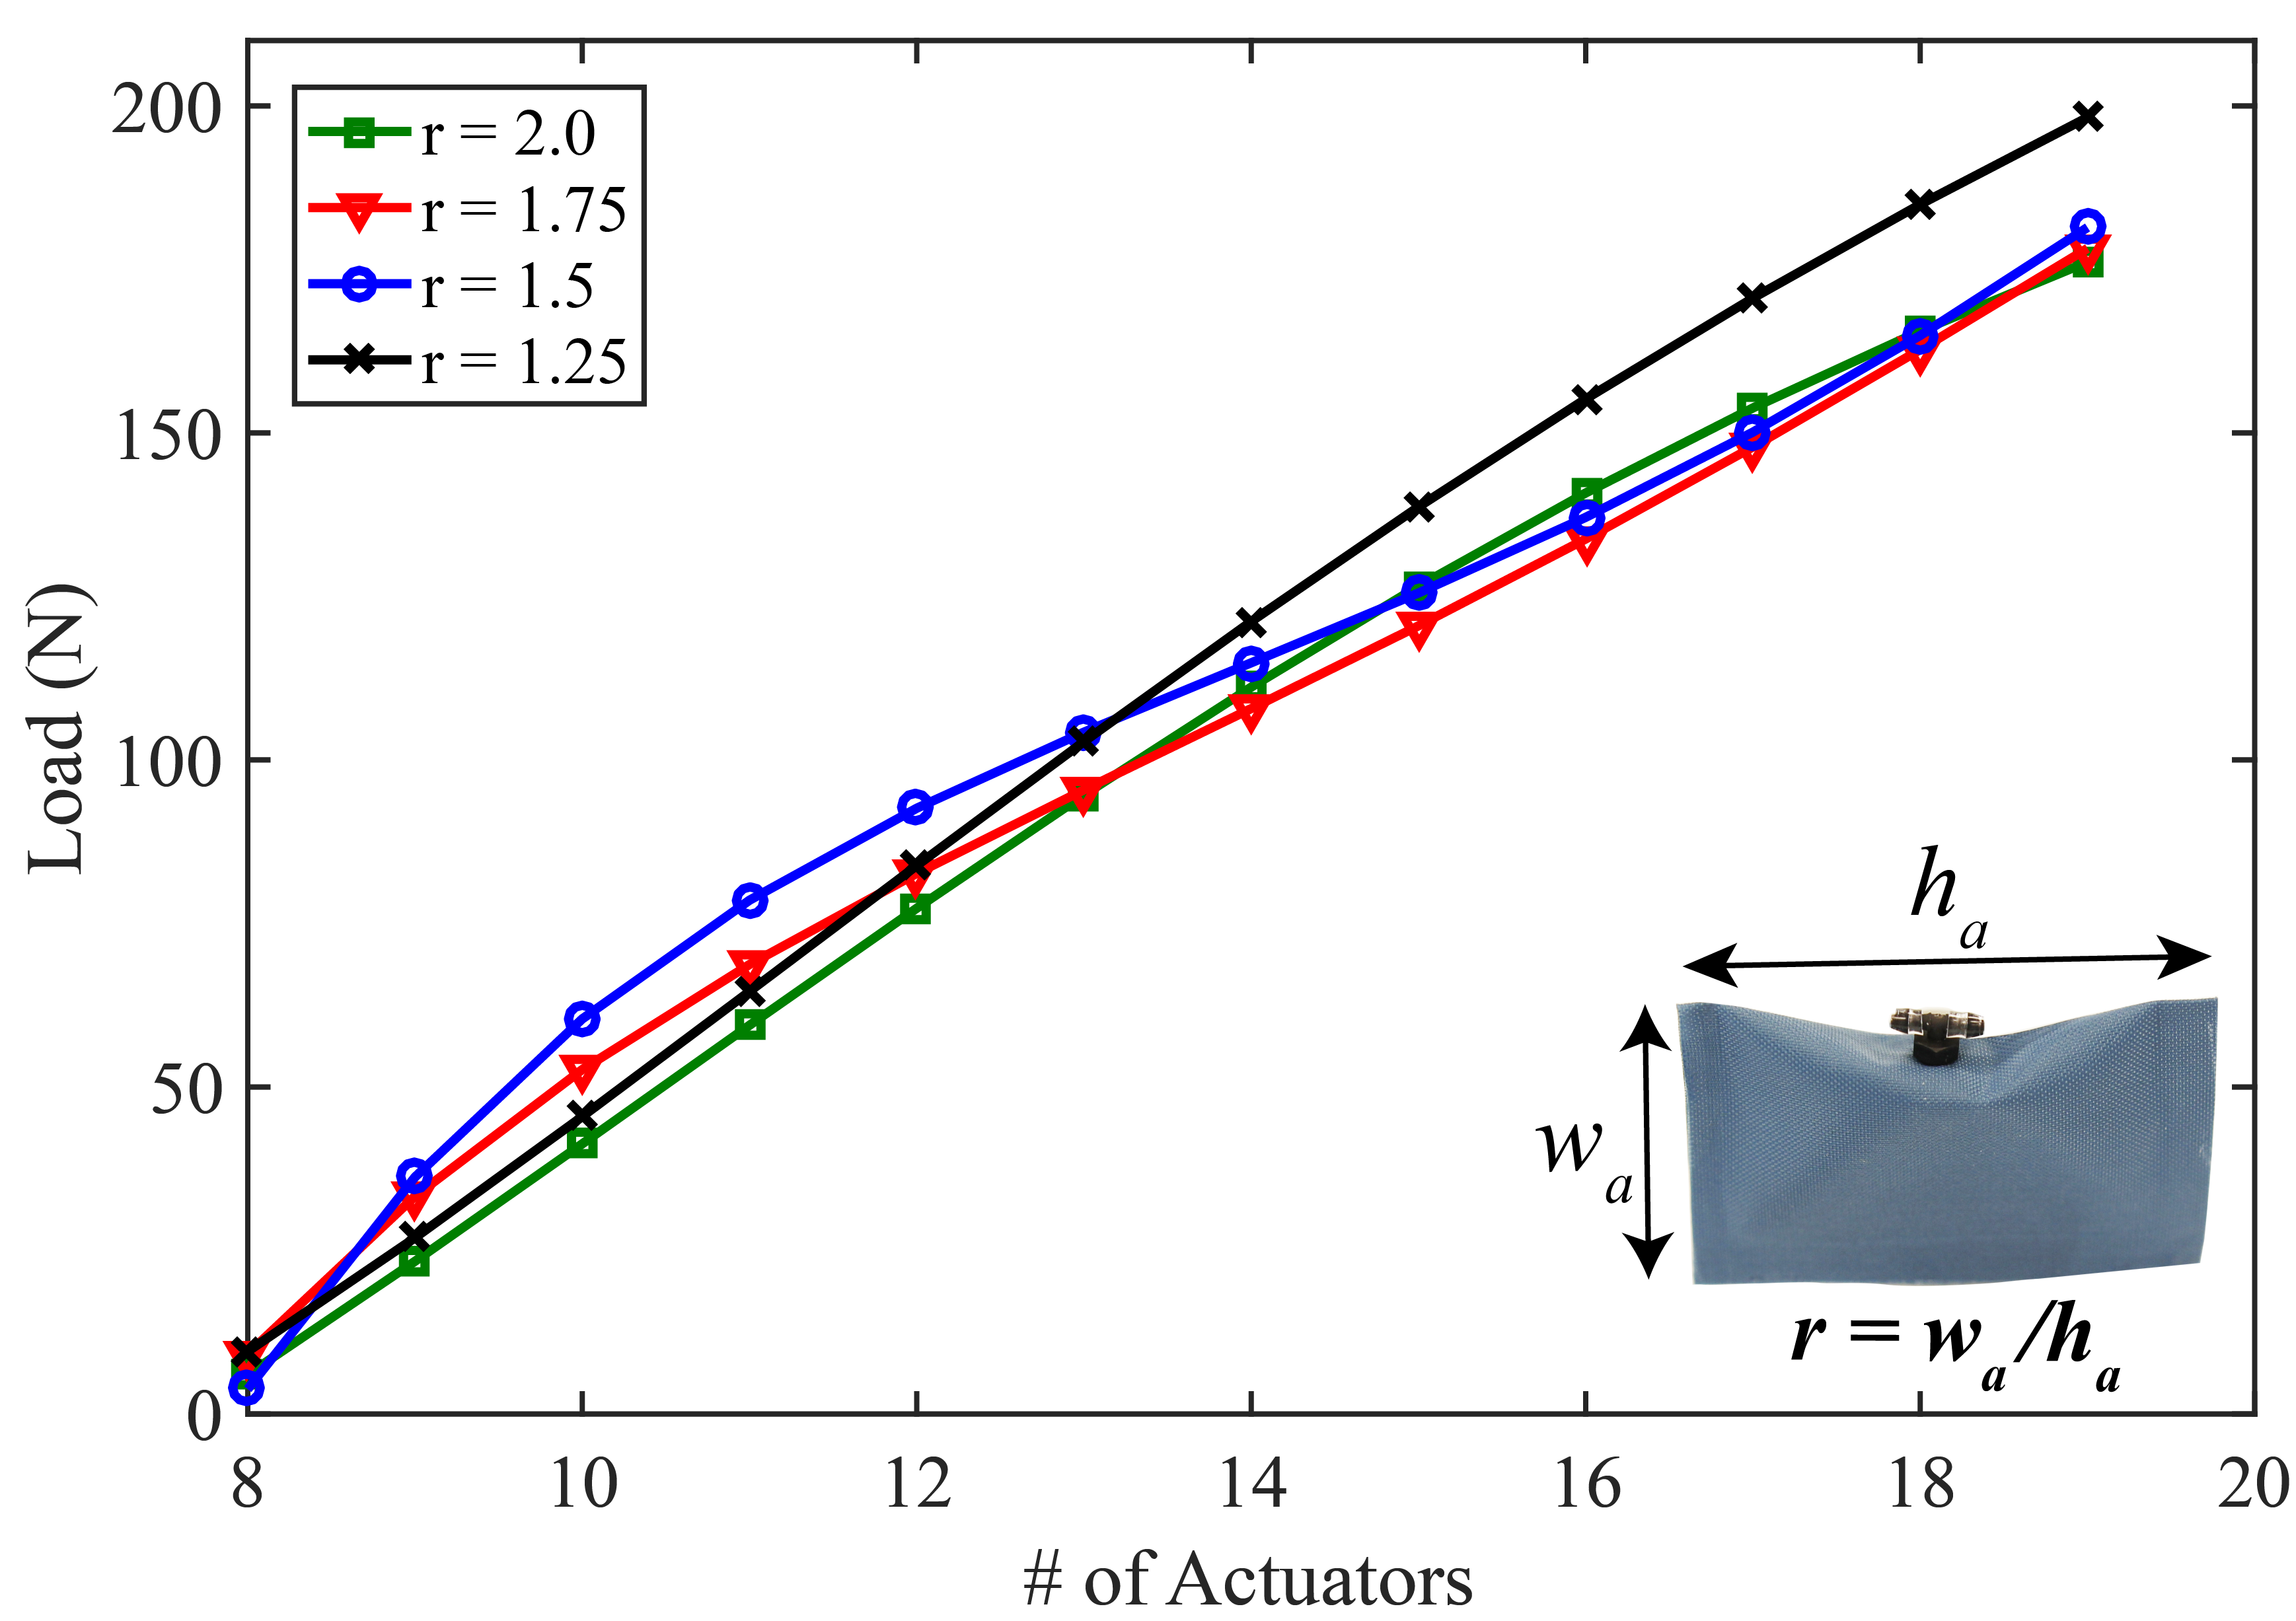
\includegraphics[width=0.48\textwidth]{Figures/fem_opti_v4}
\caption{FEM analysis of number of number of actuators and ratio (r) with regards to the force generated by bladder actuator array.}
\label{fig:fem_opti}
\vspace{-1.5em}
\end{figure}

To study the payload and bending quality of the fSPL, a set of geometrical parameters highlighted in Fig. \ref{fig:geom_param} are studied. Figure \ref{fig:geom_param}a) depicts the isometric view of a single  actuator array of length $a_{l}$, consisted of $n$ number of actuators spaced at $s_{p}$. Each actuator is consisted of 4 main geometrical parameters, the fitting length ($f_{l}$), the seal length ($s_{l}$), the active width ($w_{a}$) and height ($h_{a}$). When the actuators are inflated, it is assumed to take a circular shape and therefore the active height, $h_{a}$, becomes $\frac{h_a}{\pi}$ and all the interacting actuators create a combined bending angle of $\theta_{n}$ as seen in Fig. \ref{fig:geom_param}b). 

Figure \ref{fig:geom_param}c) shows the view of the base of a single f3CBA, where three  actuator arrays are arranged in an equilateral triangle fashion. The parameters include the circumradius of the equilateral triangle($R_{c}$), the inradius of the equilateral triangle ($R_{i}$), the width of the actuator ($w_{b}$), the height of the actuator ($h_{b}$), the active width of the actuator ($w_{a}$), and the active height of the actuator ($h_{a}$). 


\subsection{Optimization of Bladder Geometrical Parameters}
The three main geometrical parameters is studied and optimized are the active width and height of the actuators ($w_{a}$ and $h_{a}$), and the number of actuators ($n$) based on their major contribution to the bending and payload capacity of the fSPL.

The active height ($h_{a}$) contributes to the bending capability, while the active width ($w_{a}$) contributes to the stability to the actuator array. If $w_{a}$ is less than $h_{a}$ then the contact surface between consecutive actuators will be small and therefore the actuators will slip resulting in torsion effects and the incorrect distribution of force from actuator to actuator.

Therefore, $w_a$ is set to be greater than $h_a$ by a ratio $r$ that is larger that $1.0$. The active width and height are also constrained by the diameter of the fitting $f_l$ being used, which is 6.23$mm$, and the heat seam length $s_l$ created by the heat sealer, which is 5$mm$. The spacing between the actuators ($s_{p}$) is limited to above $7.5mm$ because of sewing manufacturing limitations. Both the active width and height of the actuator are also constrained by $R_{c}$, which also defines the cross-sectional radius of the fSPL, constrained to 50$mm$. The $\theta_{n}$, or the angle of the inflated  actuator array, is designed to achieve at least 180$^{\circ}$ when fully inflated. The physical constraints mentioned above are seen as follows:


\begin{align*}
R_c &= 50mm    &  s_l &\geq 5mm      &  \theta_n&=180^\circ\\
f_l&=6.23mm         &  a_l&=160mm   &  s_p&\geq7.5mm
\label{eq:constraints}
\end{align*}

Using the number of bladders ($n$), the spacing ($s_{p}$) and the active height ($h_{a}$) can be calculated as follows:
\begin{align} 
w_a &= r\cdot h_a \\
s_p &=  \frac{(a_{l} - 2\cdot(a_l/n))}{n} \\ 
h_a &=  \frac{s_p \cdot \pi}{2\cdot(1-sin(\theta_n/(2\cdot n))} \label{eq:wa_sp_ha}
\end{align}

From the circumradius ($R_c$) and inradius ($R_i$) in Fig. \ref{fig:geom_param}b), we can calculate the active width ($w_a$) as follows:
\begin{align} 
w_a &\leq  R_c/(\frac{\sqrt{3}}{6} + \frac{1}{r}) - 2\cdot s_l -f_l \label{eq:wa_ha}
\end{align}

\subsubsection{FEM Optimization of the Geometrical Parameters}

\begin{figure}[b!]
\centering
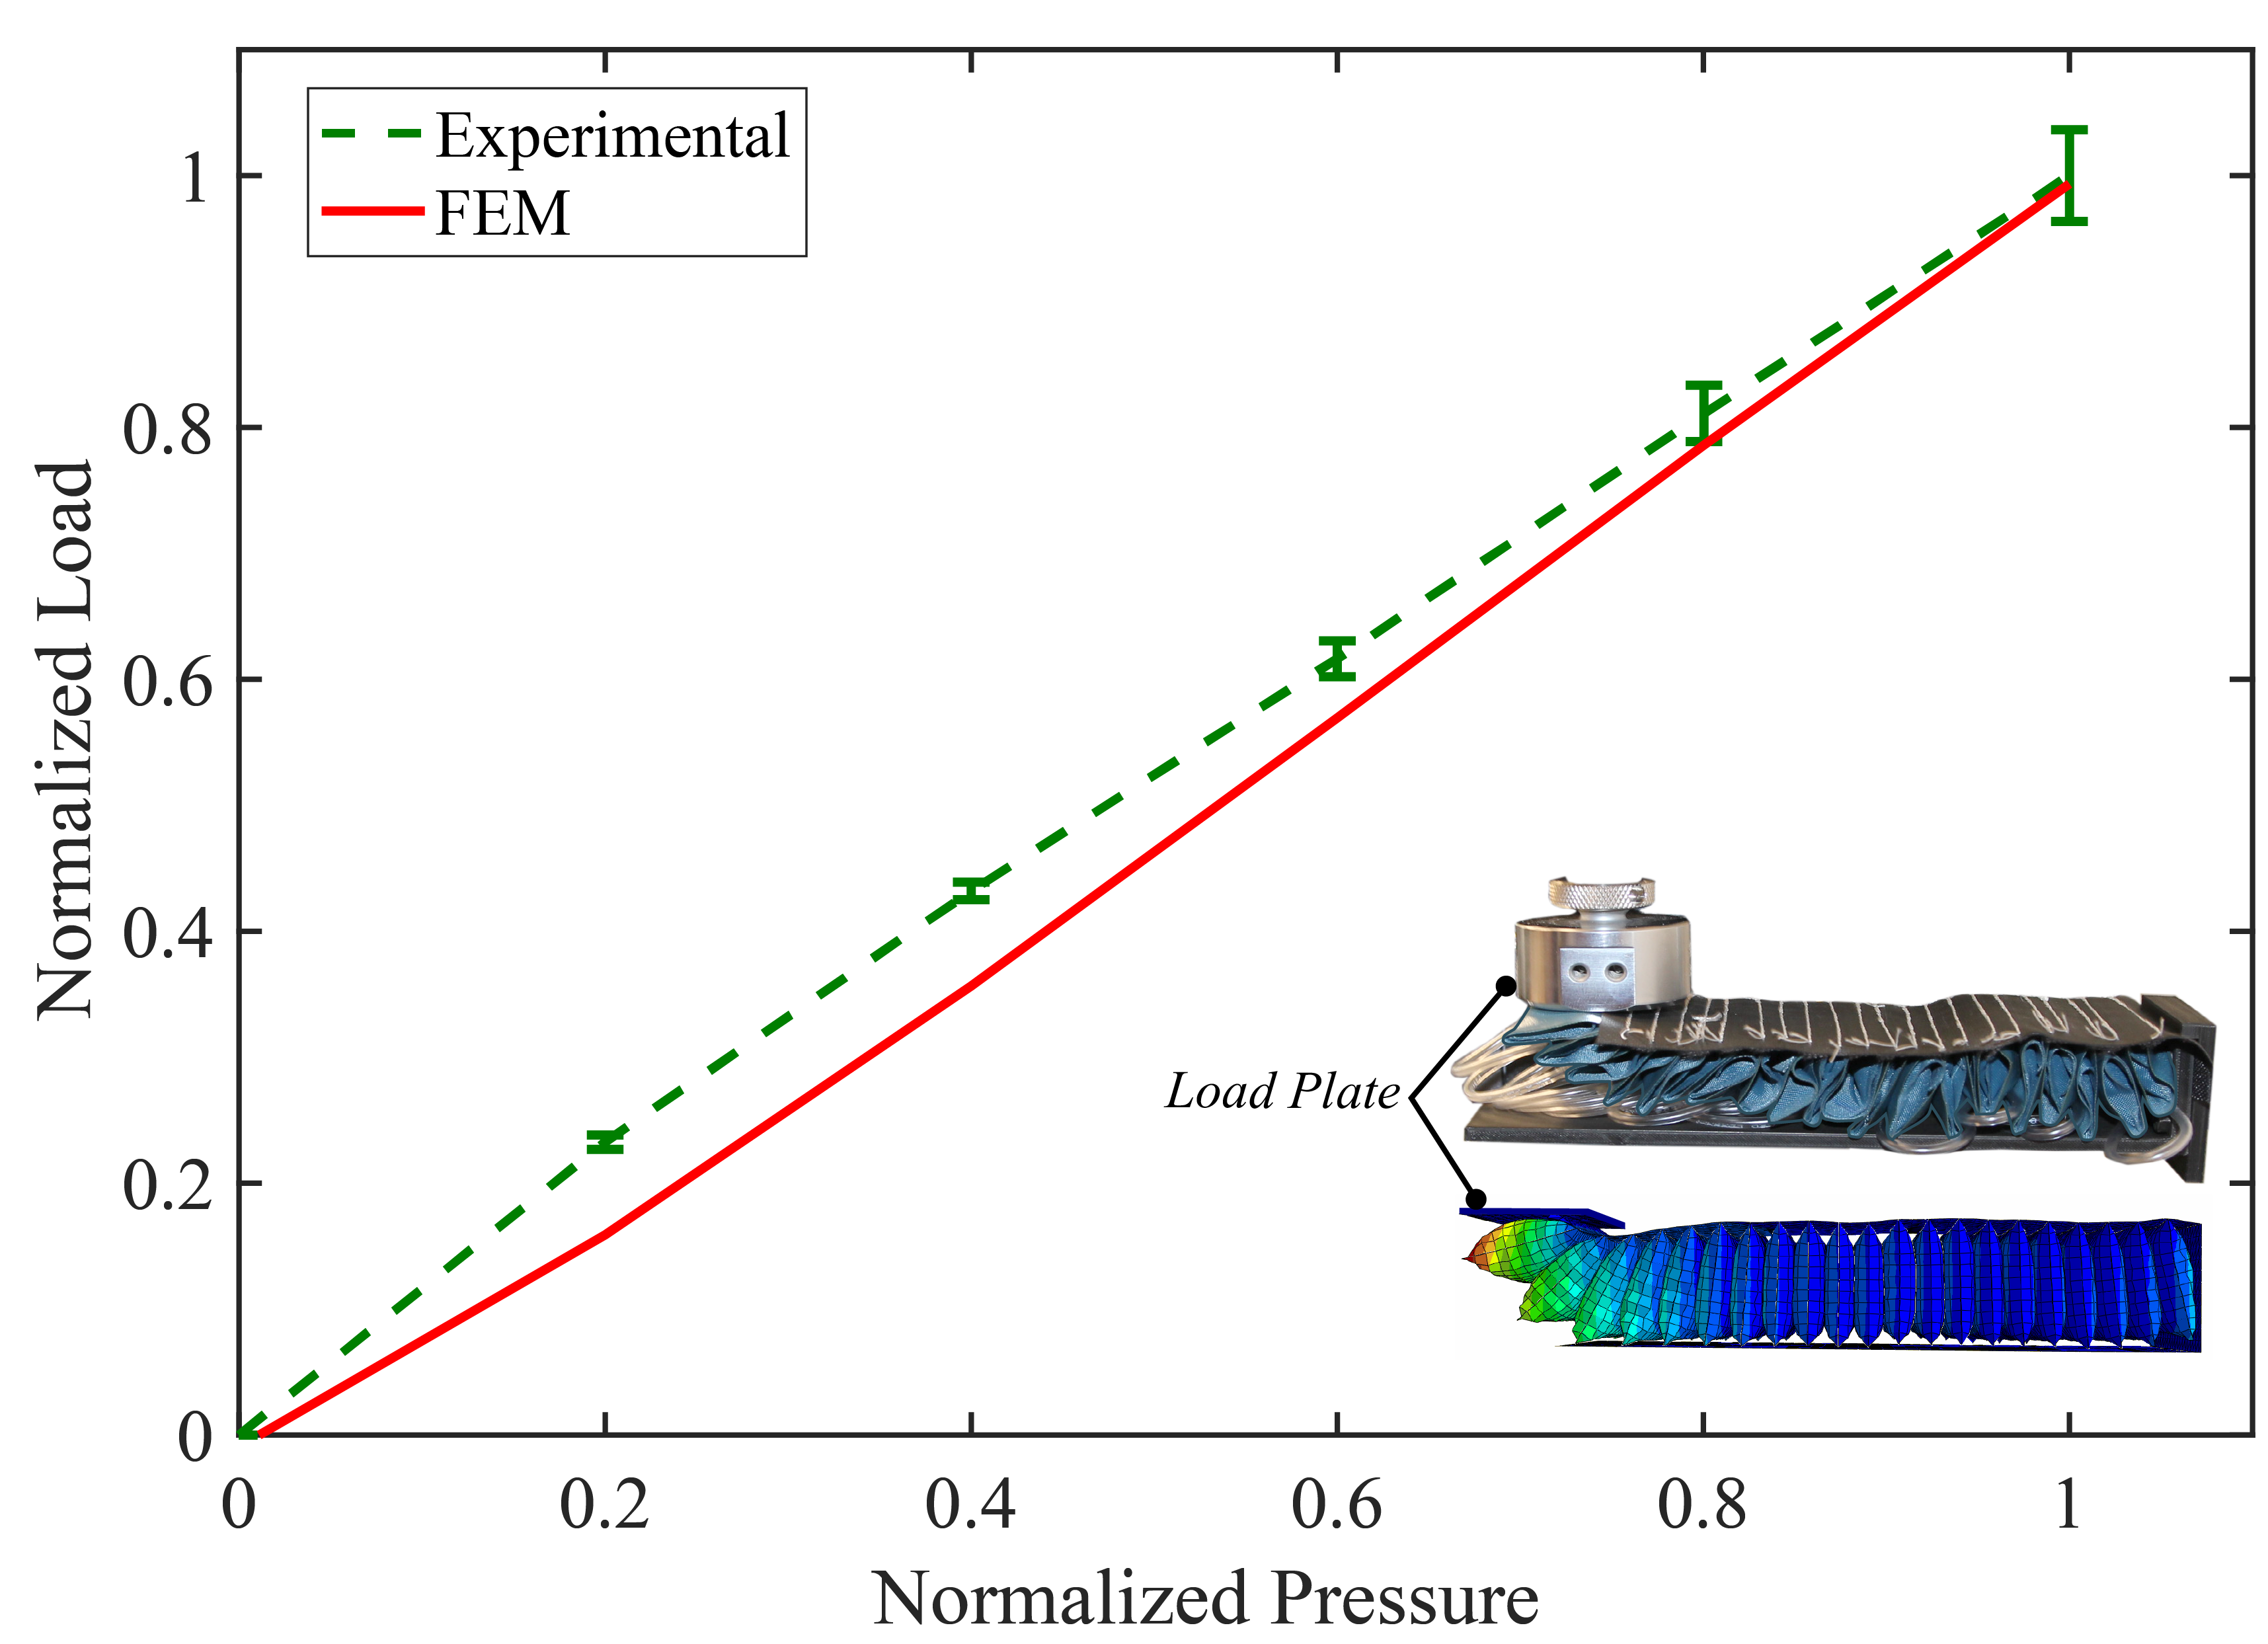
\includegraphics[width=0.45\textwidth]{Figures/single_FEM_REAL}
\caption{Payload Capability of a Single Bladder Array compared between FEM and Experimentally Validated}
\label{fig:single_fem_real}
\vspace{-1.5em}
\end{figure}

The optimization function is set as the tip force of a bending actuator array seen in Fig. \ref{fig:fem_opti}. This tip force is simulated using computational FEM model simulations with two varying parameters, the ratio ($r$) and the number of actuators ($n$). The ratio ($r$) was varied from $1.25$ to $2.0$, as seen in Fig. \ref{fig:fem_opti}. The ratio $r$ is then used to calculate $w_a$ and $h_a$ using Eq. 2 and 3. The number of actuators ($n$) is varied based off the minimum and maximum $s_p$. The maximum $n$ is determined by the minimum $s_p \geq 7.5mm$, which meant $n = 19$ determined from Eq. 2. The minimum $n$ is determined by the minimum number of actuators required to generate significant tip force from the actuator array, this was determined with FEM simulations as $n = 8$, as seen in Fig. \ref{fig:fem_opti}. As seen in Fig. \ref{fig:fem_opti}, the more the actuators in the array, the higher the tip force of the actuator array. By varying the ratio ($r$) between $w_a$ and $h_a$, we notice fairly similar trend lines for the ratios, seen in Fig. \ref{fig:fem_opti}. Therefore, the setup least likely to have actuator slippage that could result in torsion effects is selected, with $r =2.0$. Finally, in order to get the setup that produced the highest amount force, the maximum $n$ possible ($n = 19$) is chosen.

\subsubsection{Experimental Validation of the Actuator Setup}

To experimentally validate the quality of the FEM model against the performance of the bladder actuator array prototype, the payload capacity of the bladder actuator array is first evaluated for payload at different set pressures. The bladder actuator array is mounted against the force plate of the universal tensile testing machine (Instron 5944, Instron Corp., High Wycombe, United Kingdom) as seen in Fig \ref{fig:payload_all}e). The bladder actuator array is inflated upwards away from the influence of gravity and the load is measured at small pressure increments until 0.34$MPa$, as seen in Fig \ref{fig:single_fem_real}. Both FEM and experimental data demonstrated similar load output trends with an RMS error of 9.087$N$. 


\section{SPL Manufacturing/Fabrication and Integration}

\begin{figure}[t!]
\centering
\includegraphics[width=0.5\textwidth]{Figures/fabrication}
\caption{Fabrication of the fSPL. a) The bladder array when inflated. b) The CNC Process to fabricate bladders. c) Each singular bladder. d) The entire fSPL composed of 3 segments of f3CBAs.}
\label{fig:fabrication}
\vspace{-1.5em}
\end{figure}

The fabrication process of the fSPL shown in Fig. \ref{fig:fabrication} starts from creating the fabric bladders using the TPU-coated nylon fabric (6607, Rockywoods Fabric, CO) selected in subsection \ref{sec:mat_select}.  The material is cut into shape using a laser cutter (Glowforge Pro, Glowforge, Seattle, WA) and the pneumatic fittings are attached (5463K361, McMaster-Carr, Elmhurst, IL). A sealant is also added around the pneumatic fitting to prevent any air leakage (Seam Grip, Gear Aid, Bellingham, WA). The material with the fittings are then arranged on the customized CNC router (Shapeoko 3, Carbide Motion, Torrance, CA) with a soldering iron tip set at 232$^{\circ}$C and traced to seal the fabric bladders, as seen in Fig. \ref{fig:fabrication}b). This apparatus enables rapid heat-sealing of a variety of fabric soft actuator patterns of different shapes and materials accurately and repeatedly, up to 24 individual actuators at a time. Pouches for the individual actuators are then evenly sewn into an array configuration as seen in Fig. \ref{fig:fabrication}a), using a heavy duty sewing machine (Memory Craft 6500P, Janome, Hachioji, Tokyo). The individual actuators as depicted in Fig. \ref{fig:fabrication}c), are then slotted into the pouches in the actuator array, as shown in Fig. \ref{fig:fabrication}a). This approach of using individual actuators in pouches allows for ease of replacement of the actuators in the event of maintenance. Three sets of 3 actuator arrays are then arranged and sewn in an equilateral triangle fashion, with internal angles of 60$^{\circ}$, to create equilateral triangle prisms called the fabric 3-chambered bending actuators (f3CBAs) shown in Fig. \ref{fig:fabrication}d). The 3 sets of f3CBAs are connected together using 3D printed modular connectors fabricated using PLA material (1811201, MakerGear, Beachwood, Ohio). The actuator arrays are sewn and glued onto the connector pieces using kevlar threads (8800K41, McMaster-Carr, Elmhurst, IL) on both ends. The f3CBAs segments are bolted at the connector pieces to create the fSPL as shown in Fig. \ref{fig:fabrication}d). The modularity of the connector pieces also allows for the addition of a variety of end-effectors to be mounted at the tip of the fSPL such as a suction cup (5427A636, McMaster-Carr, Elmhurst, IL).

Finding the appropriate mounting point for the fSPL on the human body is essential for multiple factors such as force transmission, comfort, and safety. Keeping in consideration, the functional requirement to carry up to four times its weight, its support requires to be strong enough to hold its position. To tackle these issues the hip was used as the main attachment point for the fSPL. Mounting the fSPL at the hip also allows for free manipulation of the arm through a workspace that complements the user's arms. To attach the fSPL to the body, a modified technical belt(S\&F Deluxe Technical Belt, Lowepro, Petaluma, CA) as shown in Fig. \ref{fig:fig1}c) is used and the modifications are focused on increasing the belt's resistance to force. The utility belt includes reinforcement necessary to distribute the forces generated by carrying weights ranging from 0.1$kg$ to 1$kg$. A zippered fabric pouch used to house the fSPL in a compressed state for ease of storage. A support structure consisting of a 3D printed “L” bracket is designed to mount the fSPL to the belt. A thermoplastic acrylic-polyvinyl chloride (TAPC) sheet manufactured to fit the curvature of the torso is used as a padding structure to evenly distribute the forces onto the body to avoid pinch points and discomfort.

\section{Testing and Evaluation of fSPl}
For the fSPL to be effective in everyday use, it is vital that the fSPL is capable of carrying the desired payload and maneuver effectively in 3D space. Therefore, we evaluated the fSPL through experimentally validating the computational FEM models of the system, performing various payload experiments, determining the maneuverable workspace of the SPL, and finally determining the users' ability control and carry a variety of daily livings objects through pick-and-place experiments.

\subsection{FEM vs Experimental}

%Why are there two FEM vs Experimental sections here?
\subsubsection{f3CBA FEM vs Experimental}

\begin{figure}[b!]
\centering
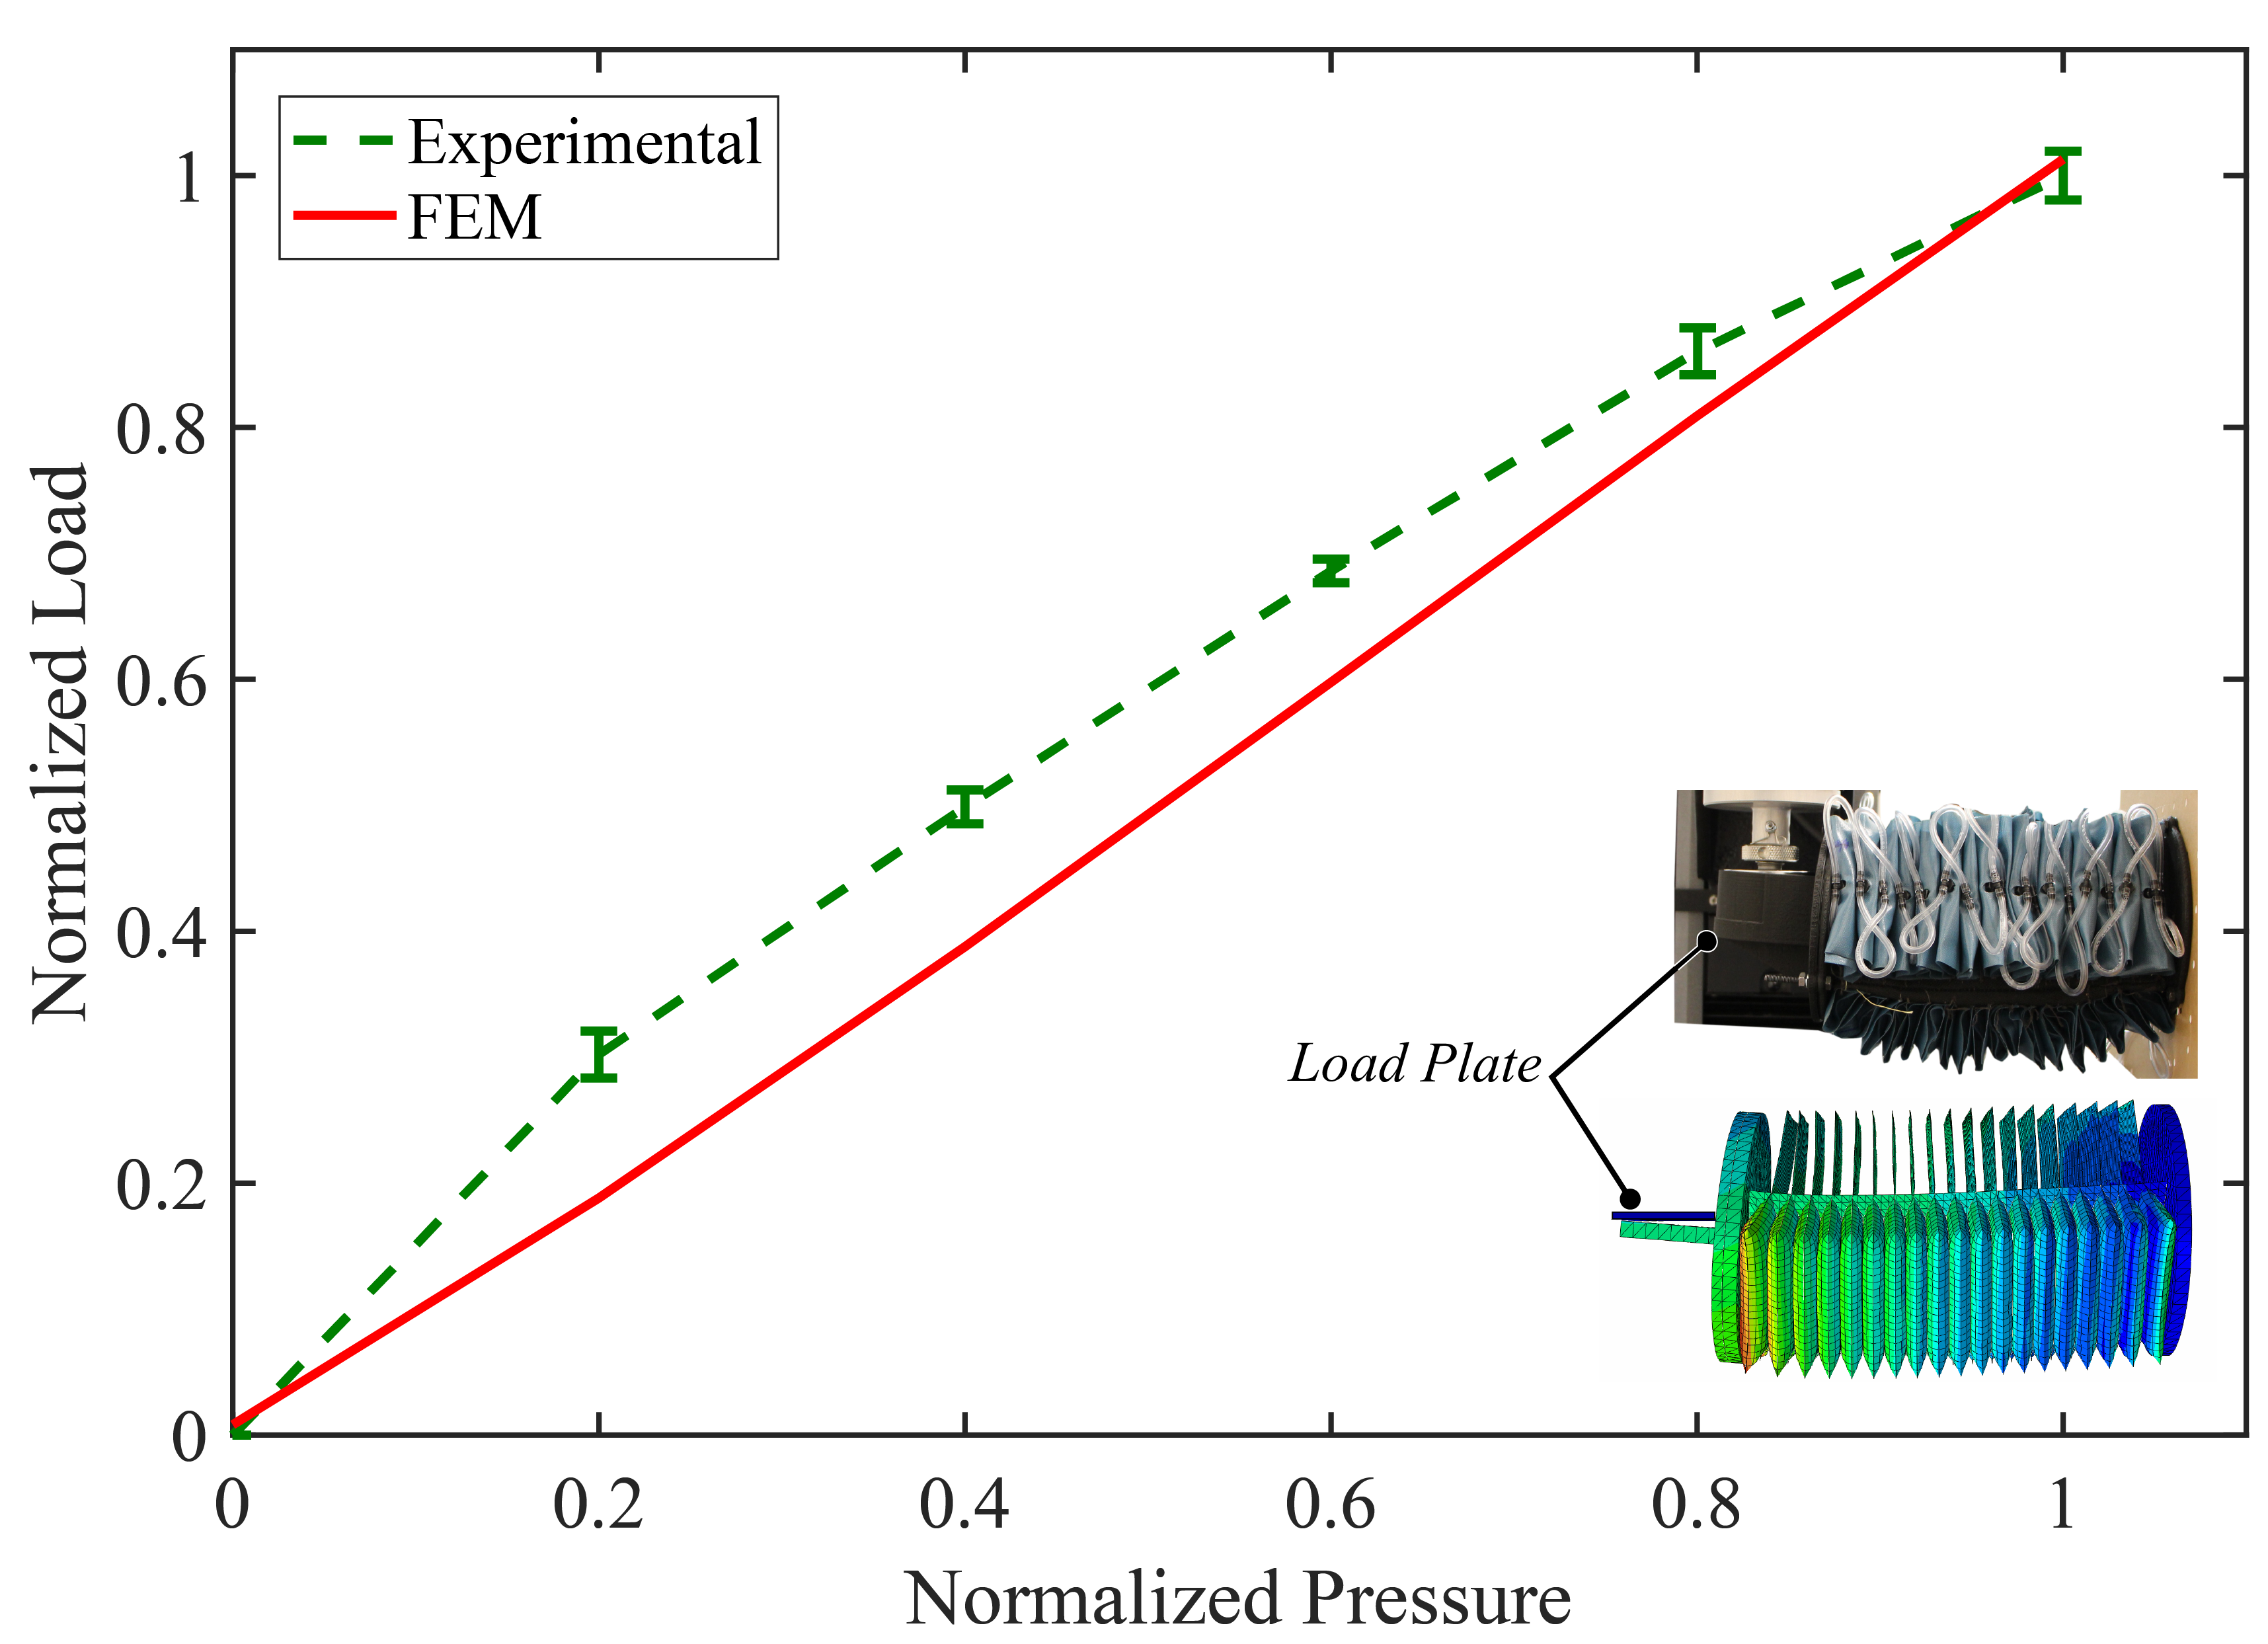
\includegraphics[width=0.45\textwidth]{Figures/3CA_instron}
\caption{Payload Capability of a f3CBA unit compared between FEM and Experimentally Validated}
\label{fig:f3CAs_load_fem_real}
\vspace{-1.5em}
\end{figure}

A single f3CBA segment is also mounted against the UTM as seen in Fig. \ref{fig:payload_all}a). This was done to compare the load capacity when inflating 2 adjacent bladder actuator arrays against the FEM model of the same set up. The two sides of the f3CBA were also inflated until 0.34$MPA$, as seen in Fig. \ref{fig:f3CAs_load_fem_real}. Both the experimental and FEM simulation data when compared showed close approximation with an RMS error of 4.057$N$. 

\begin{figure}[t!]
\centering
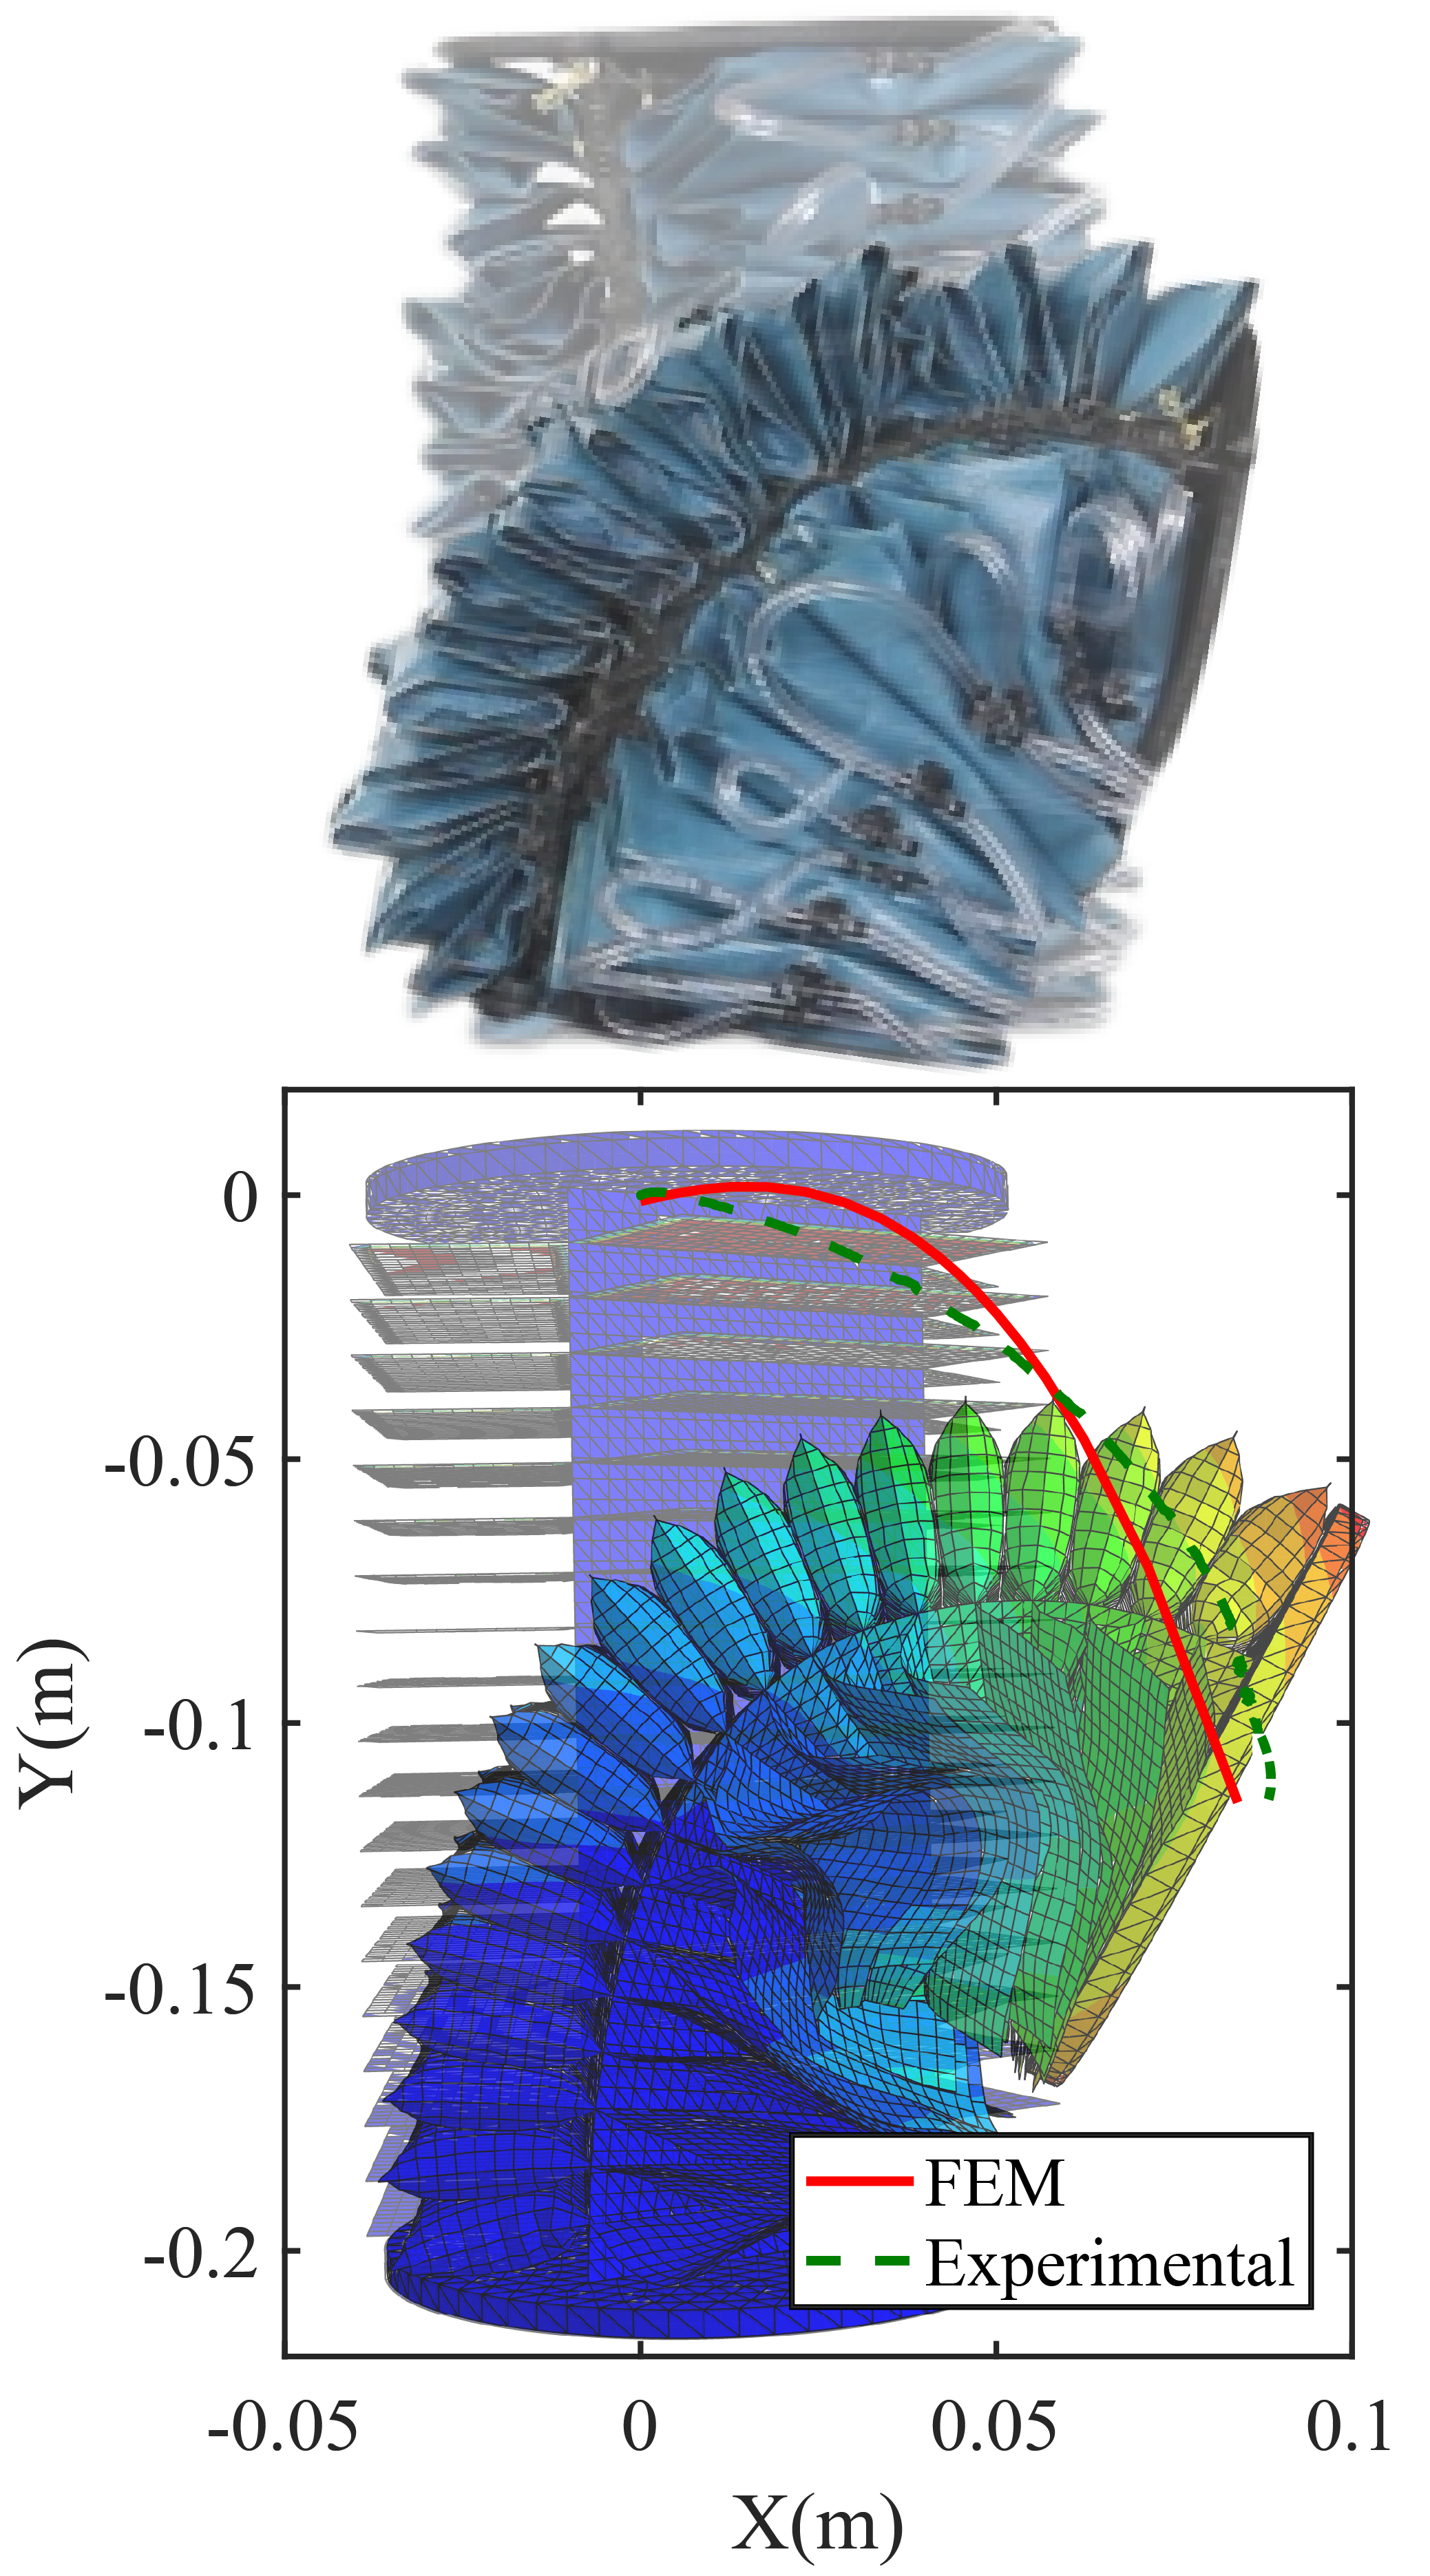
\includegraphics[width=0.43\textwidth]{Figures/3CA_bend_FEM_REAL_v2}
\caption{Bending Capability of a f3CBA unit compared between FEM and Experimentally Validated}
\label{fig:f3CAs_bend_fem_real}
\vspace{-1.5em}
\end{figure}


An experiment to compare the bending motion trajectory of a f3CBA segment of the FEM model and prototype was also conducted. A set of passive reflective markers are attached to the distal end of the segment to create a rigid body in the center of the distal enter and the motion capture system is used to track the motion of the distal end when one side of the segment is inflated up to 0.345$MPa$ quasi-statically, as seen in Fig. \ref{fig:f3CAs_bend_fem_real}. The distal end position of the 3CA in the FEM simulation and experimental results in a Euclidean distance error of 6.8$mm$. The rather close match between the trajectories of the model and experimental data shows that the FEM model can be used to predict the complex motion of a single segment of the fSPL.

\subsubsection{fSPL FEM vs Experimental}

To investigate the payload capacity of the complete 3-segment, fSPL using the prediction of the FEM model and the experimental validation through the fSPL prototype, the fSPL was inflated away from gravity and the end-effector of the fSPL was pushed against the UTM load plate as seen in Fig \ref{fig:payload_all}c). The maximum load detected from the instron force plate was 1.5$kg$ where the bottom adjacent chambers of the distal segments were pressurized up to 0.345$MPa$ and the proximal segment’s bottom adjacent chambers were pressurized up to 0.207$MPa$ to maintain the fSPL parallel the ground against gravity. Both FEM and experimental data demonstrated similar load output trends with an RMS error of 9.087$N$. 

Finally, we determine the FEM’s model to predict the continuum complex non-linear motion produced by the entire fSPL, a single complex pose is generated and recorded using the motion capture system. Four sets of markers were added at the proximal and distal end of every segment to create virtual rigid bodies along the body of the fSPL. The fSPL was mounted horizontally against gravity, and the bottom two chambers of the first segment were inflated to 0.207$MPa$ and 0.345$MPa$ respectively, the bottom right chamber of the second segment was inflated to 0.207$kPa$, and finally the bottom left chamber of the third segment was inflated to 0.207$MPa$ to generate a snake-like motion using the fSPL, as seen in Fig. \ref{fig:pose}. The experimental Euclidean displacement error is found to be \textbf{xxx} $mm$ when comparing the FEM model. Thus proving that the FEM models created for the single bladder actuator array, the f3CBA, and the full fSPL are able to predict the load capability and complex motions generated by the interacting bladder actuator arrays.

\begin{figure}[t!]
\centering
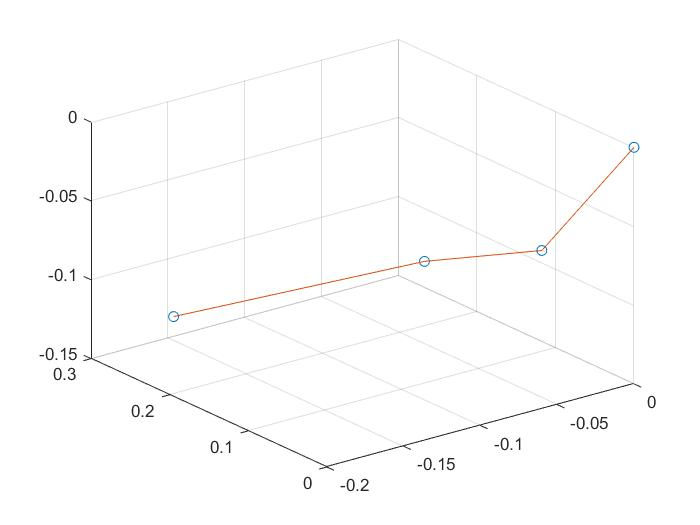
\includegraphics[width=0.45\textwidth]{Figures/SnakePose.jpg}
\caption{PLACEHOLDER Comparison of the FEM prediction of an arbitrary pose vs the resulting pose recorded via motion capture}
\label{fig:pose}
\end{figure}



\subsection{Payload Capacity of the fSPL}


\begin{figure}[t!]
\centering
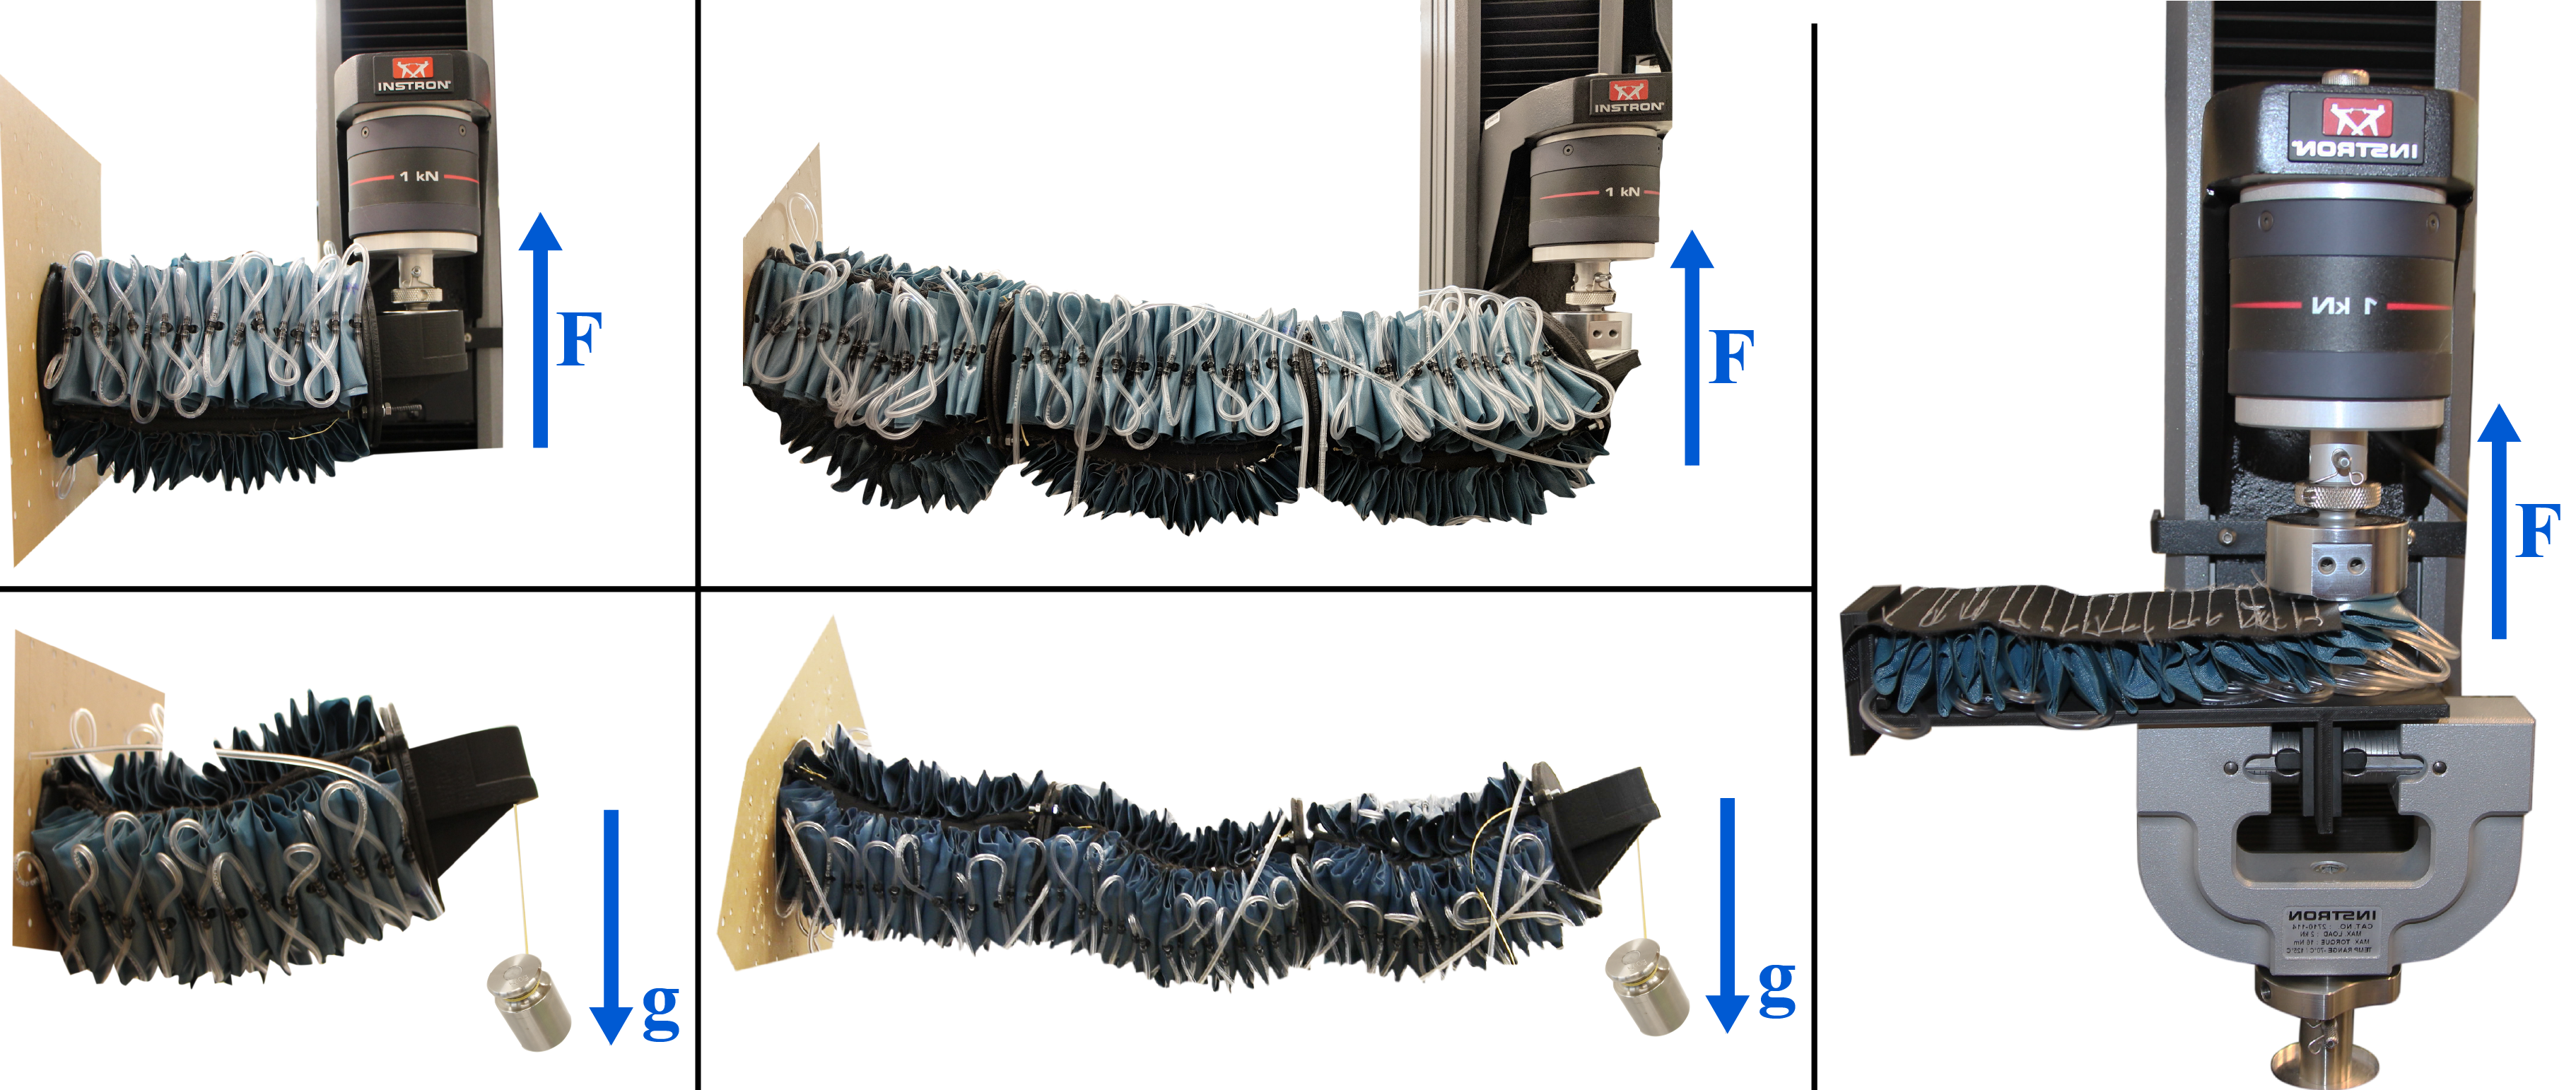
\includegraphics[width=0.45\textwidth]{Figures/payload_all_v2}
\caption{Payload Setup for single bladder array, f3CBA, and fSPL}
\label{fig:payload_all}
\vspace{-1.5em}
\end{figure}


\subsubsection{Single Bladder Actuator Array Payload}
The upward force generated by a single actuator array is tested using the Instron machine. The last actuator on the array is placed directly under the Instron machine and the air pressure inside the bladders were increased in increments of 0.069$MPa$ until 0.345MPa. In the end, the single bladder array produced 174.73$N$ of force at 0.345$MPa$, which is similar to lifting 17.4$kg$ of weights by only a single array of bladders.

\subsubsection{Single Segment f3CBA Payload}

A single arm segment was fixed horizontally and weights were then attached on the free end of the arm in increments. The bladders on the arm were then inflated until the arm segment was at least parallel with the ground. The first test was conducted by inflating only 1 side of bladders which managed to lift up 4.8$kg$ at 0.35$MPa$. Next, 2 sides were inflated which managed to lift up 6.3$kg$ at 0.372$MPa$. With the single segment weighing in at about 0.37$kg$, and able to lift up to 6.3$kg$, this means that it can carry approximately 17 times its own weight. The segment was then fixed horizontally and this time the free end was placed directly under the Instron machine. Only 1 side of bladders were inflated, which applies normal force onto the Instron machine. The air pressure was increased in increments of 0.069$MPa$ until 0.345$MPa$ and the respective force values were recorded. The test was conducted 3 times to ensure the most accurate results. At 0.345$MPa$, the segment, with only 1 side inflated produced 40.2$N$, which is equivalent to 4.02$kg$ of weight. The same procedures were repeated for when 2 sides were inflated and the segment generated 53.7$N$ at 0.345$MPa$, which is equivalent to 5.37$kg$. These results for 1 and 2 sides are very similar to the real payload test with discrepancies of only 16.7\% and 14.8\% respectively. This has shown that the single segment (f3CBA), which is able to generate 53.7$N$ of force while only weighing at 0.37$kg$ has an impressive payload-to-weight ratio of 14:1.

\subsubsection{fSPL Payload}
The arm is fixed parallel to the ground and weights were attached on the free end. The air pressure inside the bladders were increased until the arm is able to lift up the weights. The maximum payload capacity of the full arm (fSPL) is 1.5$kg$ when the first and second segment are at 0.345$MPa$ and the third segment is at 0.207$MPa$. The full arm weighs approximately 1.11$kg$, and is able to lift weights of up to 1.5$kg$.Next, the full arm was fixed horizontally and its free end was placed under the Instron machine. Air pressure in the bladders for each segment was increased gradually until all of the segments were at 0.345$MPa$, which generated a maximum force of 15.56$N$. This is comparable to lifting weights of almost 1.5$kg$ and these results show that the fSPL can carry items 1.36 times its own weight.

\subsection{Pick and Place}



\begin{figure}[b!]
\centering
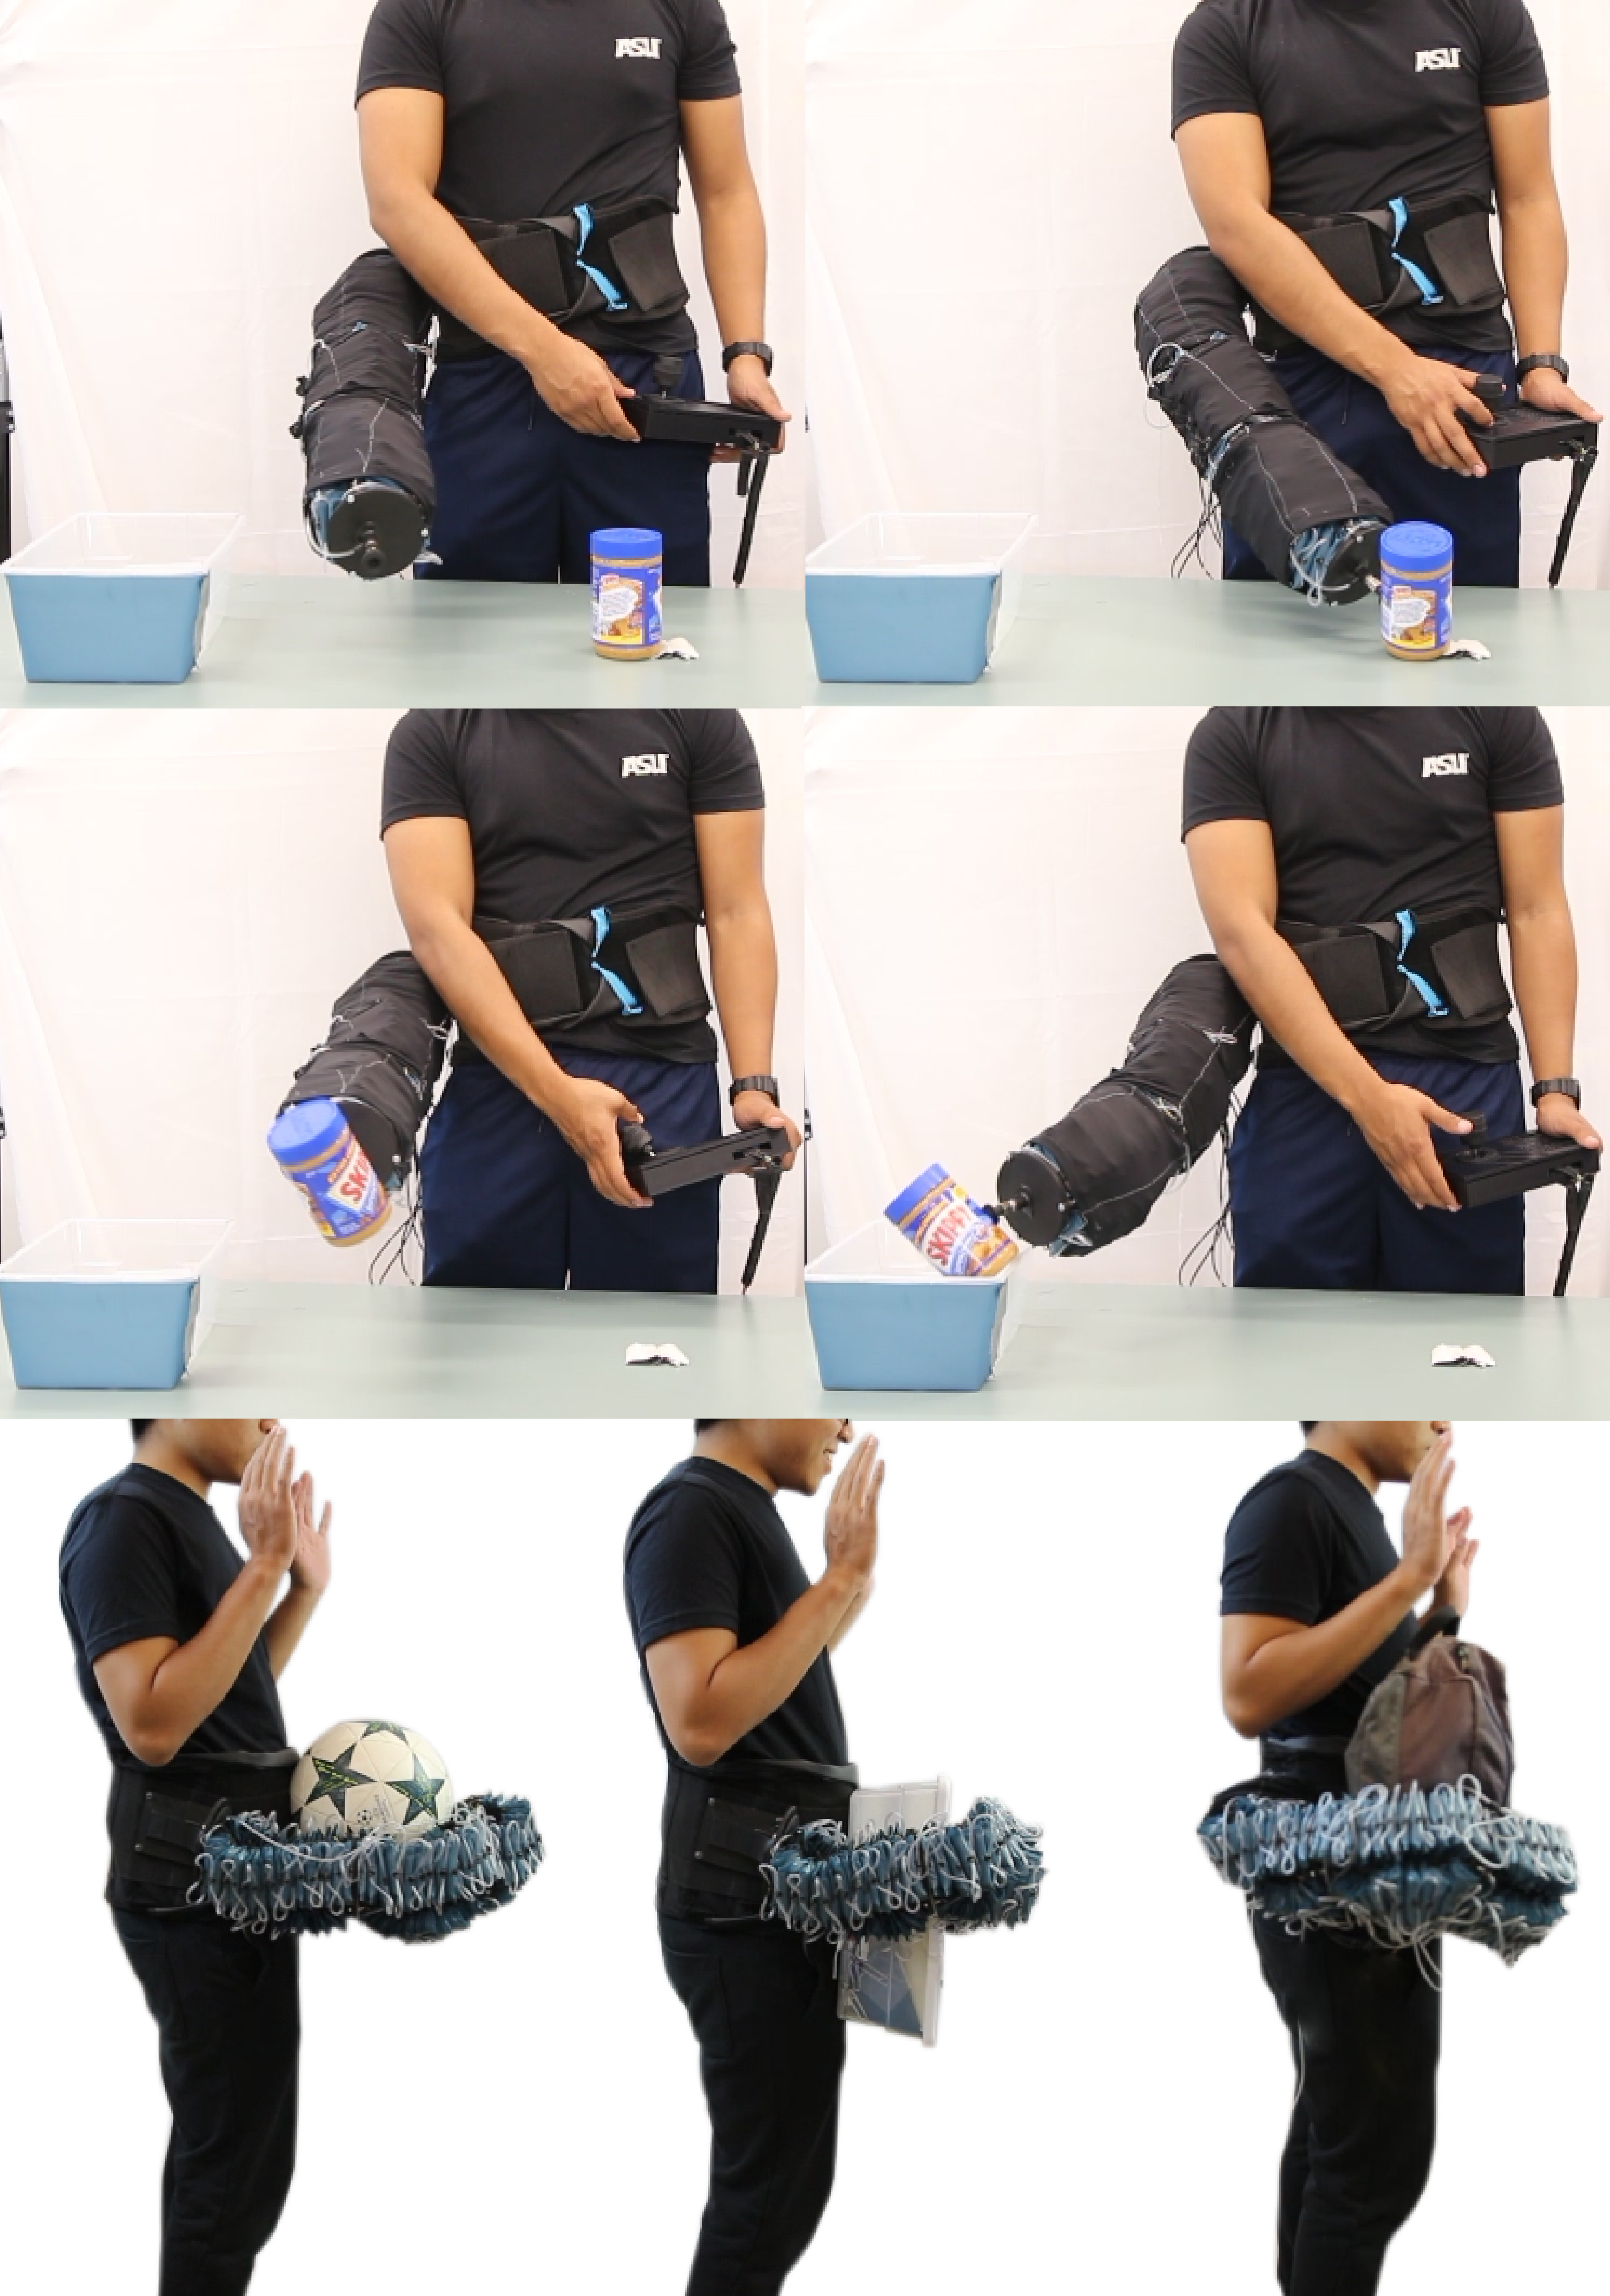
\includegraphics[width=0.45\textwidth]{Figures/pick_place_whole_body}
\caption{The different methods the fSPL can carry payload, either using its end-effector or whole body to wrap around objects.}
\label{fig:pick_place_whole_body}
\vspace{-1.5em}
\end{figure}

To test the combination of effective fSPL payload, or the payload when the fSPL is used in real-life situations, along with user controllability, a pick-and-place experimental setup designed for multiple users was designed. For this test, a vacuum suction cup manipulator is connected to the end of the fSPL. The vacuum suction cup has a theoretical payload of 0.86$kg$ and is connected to a vacuum pump with depressurization rates at 1.42x10$^{-3}m^3/s$. The experiment is set up for the user to operate the fSPL using the joystick controller to grab a jar of peanut butter (0.1$kg$) on end of the table and move it across the table where a target box (0.33x0.16x0.12$m$) is placed 0.45$m$ away from the jar, as seen in Fig. \ref{fig:pick_place_whole_body}. Three users are timed to get the jar from one end of the table into the box. Each user had 5 timed trials. User 1 improved their time from 53.28$s$ to 24.70$s$, user 2 improved from 45.34$s$ to 20.79$s$, and finally user 3 improved their time from 27.69$s$ to 17$s$. Thus proving the gradual improvement of adoption of using and controlling a soft, external limb. A variety of other daily livings objects were also successfully picked and placed, including a hair spray can (0.43$kg$) and a water bottle 0.88$kg$.


% \subsubsection{Fold and Unfold}
% Our preliminary designs show that such compliant segment is able to linearly collapse two times its own length when squeezed, but also linearly deploy and perform multi-degree-of-freedom bending motions when pressurized (Figure 14).


% \begin{figure}[t!]
% \centering
% 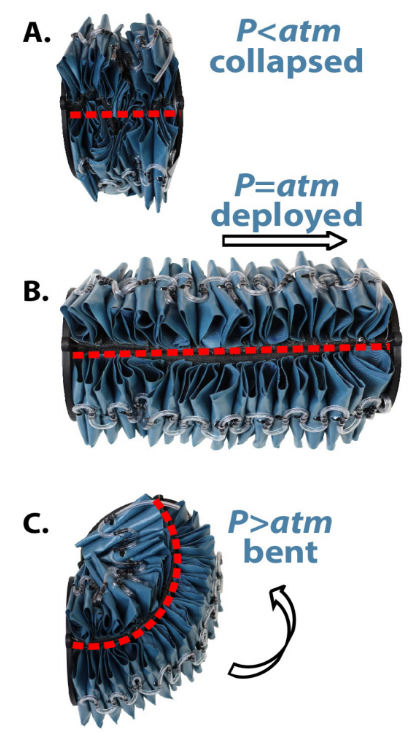
\includegraphics[width=0.30\textwidth]{Figures/unfold_fold}
% \caption{ Side view of soft fabric segment comprised of three bending
% soft fabric bundles in a triangle formation, able to collapse four 
% times its length and bend in multi-DoF when deployed and ressurized.}
% \label{fig:unfold_fold}
% \vspace{-1.5em}
% \end{figure}


\subsection{Whole-Body Continuum Grasping}


The fSPL is capable of grasping objects by wrapping itself around the objects, similar to how an elephant can grasp objects with its trunk. This method of grasping allows the fSPL to carry heavier objects than it can support at the end of the arm. The fSPL was attached to a belt worn by a user and the arm was inflated to wrap around various objects to demonstrate its whole body grasping capabilities. The user would place the object within the fSPL's reach,then the fSPL would wrap around the object to hold it in place, and the user would release the object and show that the fSPL was capable of holding the object without any other assistance. The objects held in this way were a soccer ball weighing 0.45$kg$, a full plastic storage box weighing 1.75$kg$, and a weighted backpack, as seen in Fig. \ref{fig:pick_place_whole_body}. The maximum full body carrying weight of the fSPL was tested by adding weights to the backpack until the fSPL was no longer capble of supporting the backpack. The maximum weight that the fSPL could support in this manner was 4.51$kg$.


\subsection{Workspace}
\begin{figure}[t!]
\centering
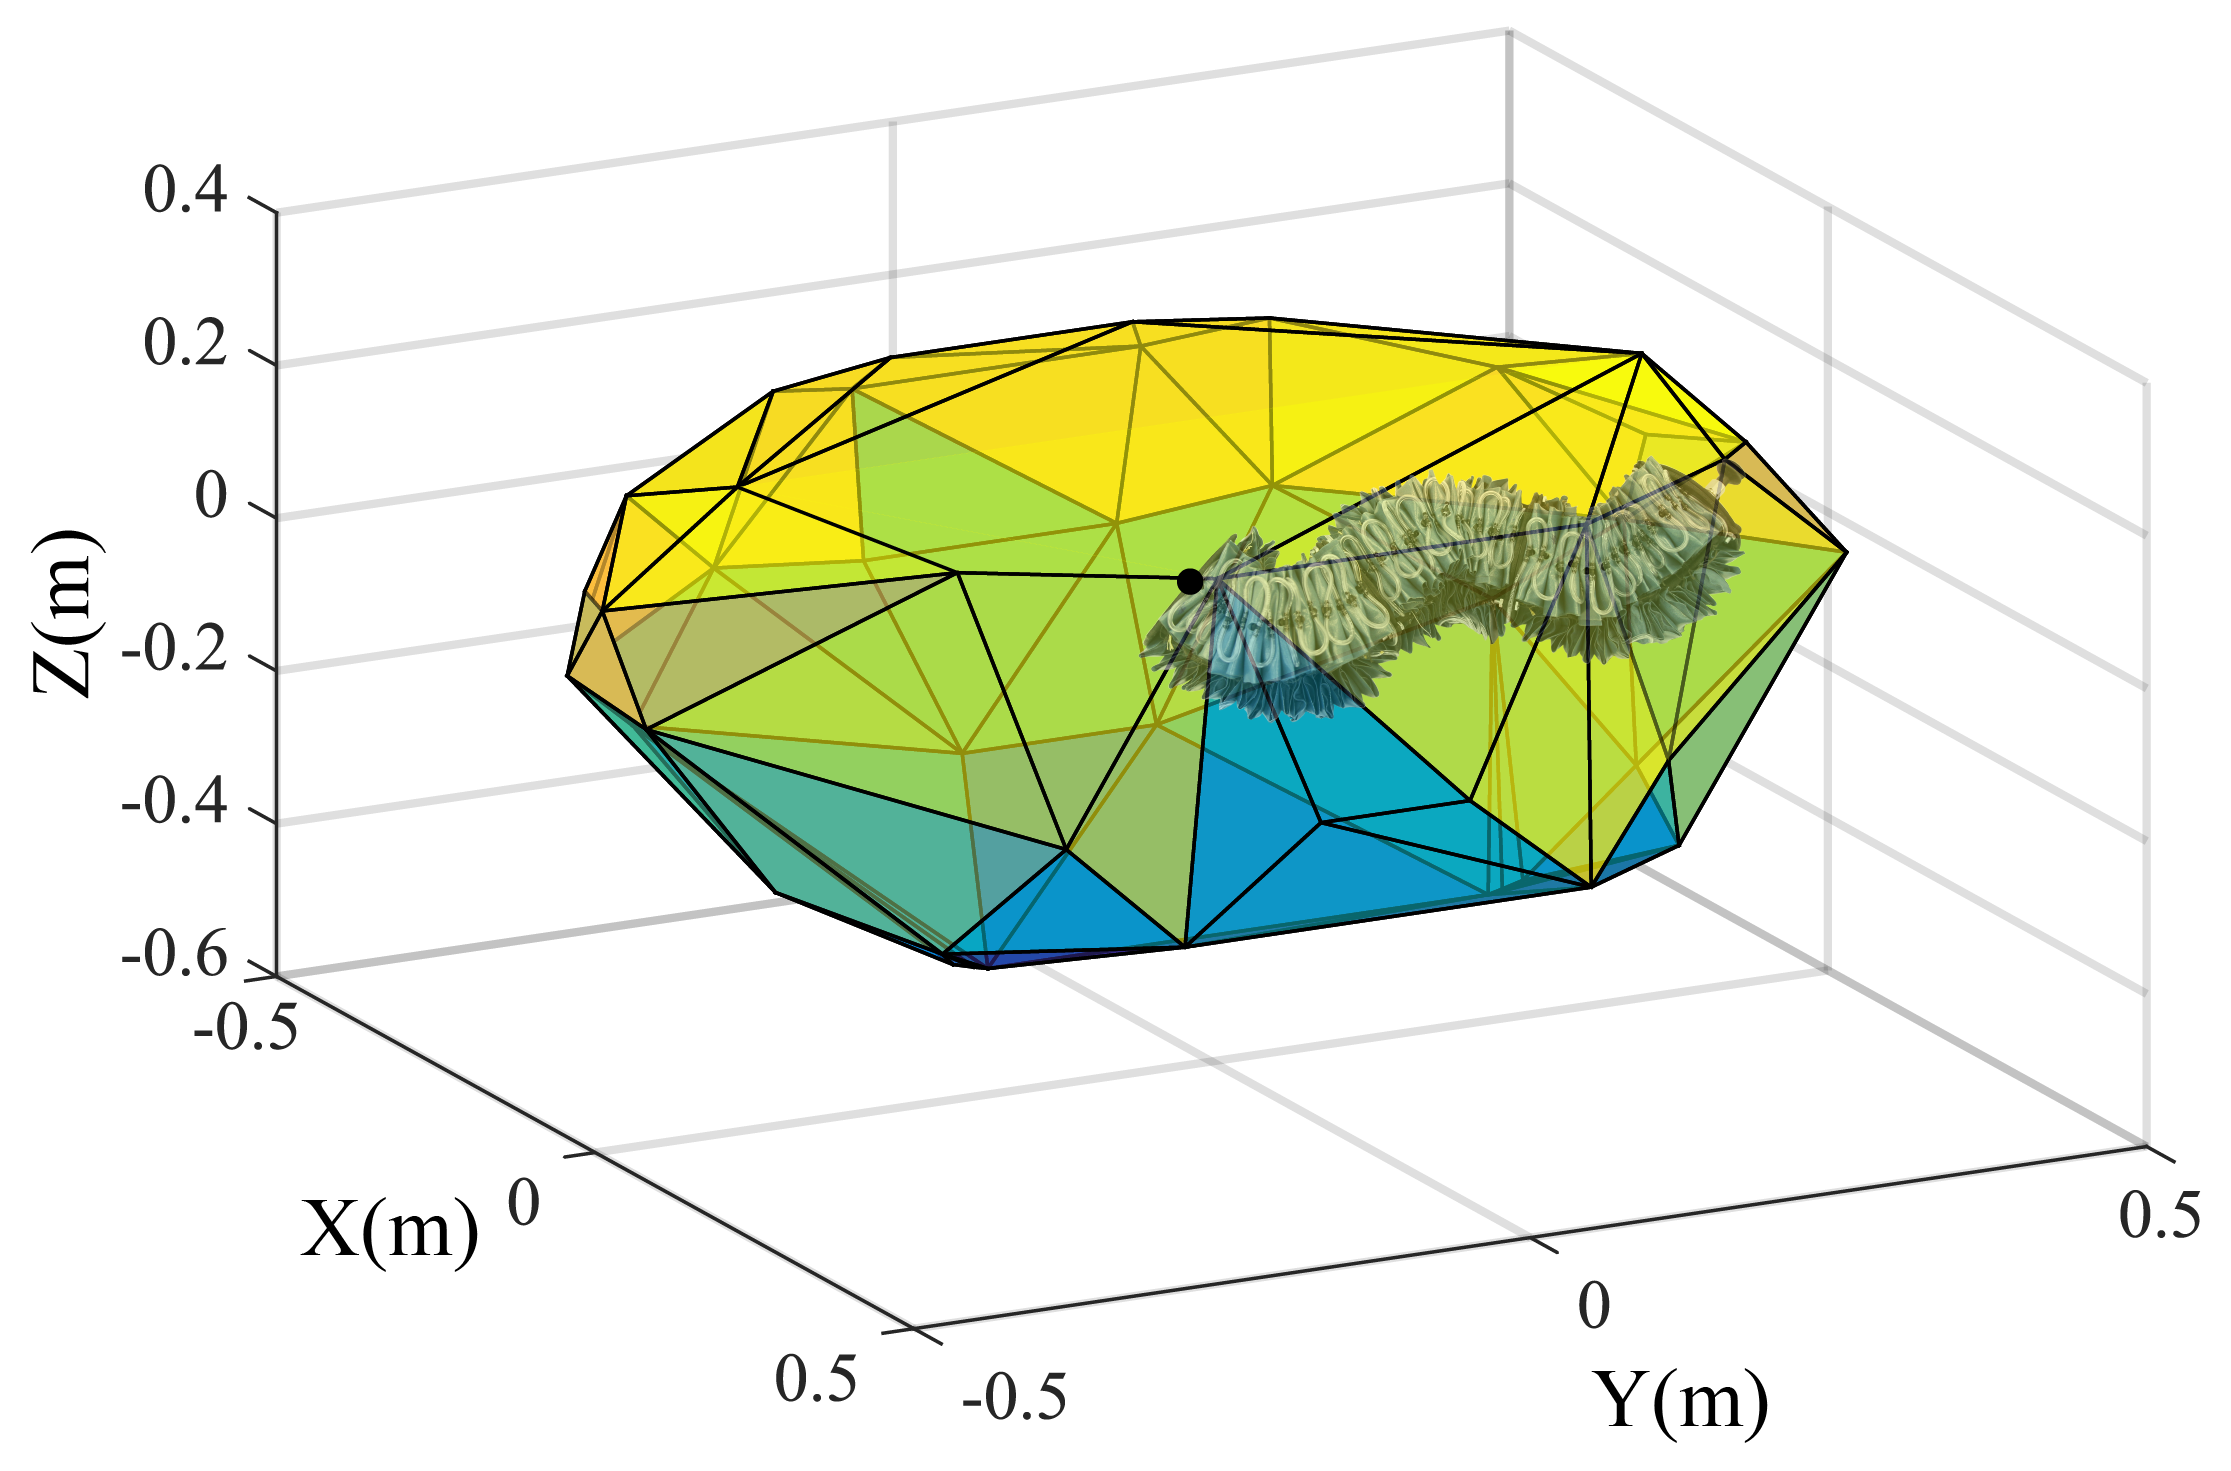
\includegraphics[width=0.45\textwidth]{Figures/Workspace_Fabric_ARM}
\caption{The different methods the fSPL can carry payload, either using its end-effector or whole body to wrap around objects.}
\label{fig:workspace_fabric_arm}
\vspace{-1.5em}
\end{figure}

The workspace of the fSPL was determined by recording the 3d coordinates of points on the outside of the workspace. The fSPL was mounted on a testing platform such that the fSPL was parallel to the floor when linearly extended, and reflective markers were placed on the base and tip of the fSPL to mark its starting and ending locations. Individual chambers of the arm were inflated to pressures up to 0.345$MPa$ to produce orientations at the maximum range of the fSPL. The pressures were provided by the testing rig which was equipped with a set of 16 regulators ((ITV1050-21N2CL4 Pressure Regulators
SMC) and 32 solenoid valves (MHE3-MS1H-3/2G-1/8-
K, Festo, Esslingen, DE). The regulators and solenoids were driven with a real time controller (CompactRIO, National Instruments Inc., Austin, TX). The position of the markers was recorded using a motion capture system with six cameras (Optitrack Prime 13W, NaturalPoint Inc., Corvallis, OR) surrounding the fSPL to produce a set of three dimensional points at the edge of the fSPL's workspace. A dome, shown in Fig \ref{fig:workspace_fabric_arm} was created from the set of points collected by the motion tracking system to represent the far reaches of the fSPL's workspace. It was assumed that the fSPL could reach any point inside that maximum dome, therefore the volume of the dome would be equal to the volume of the workspace. The fSPL has a workspace volume of 0.22m$^{3}$, a maximum vertical range of 0.63$m$ and a maximum horizontal range of 0.65$m$. 





% \begin{figure}[t!]
% \centering
% 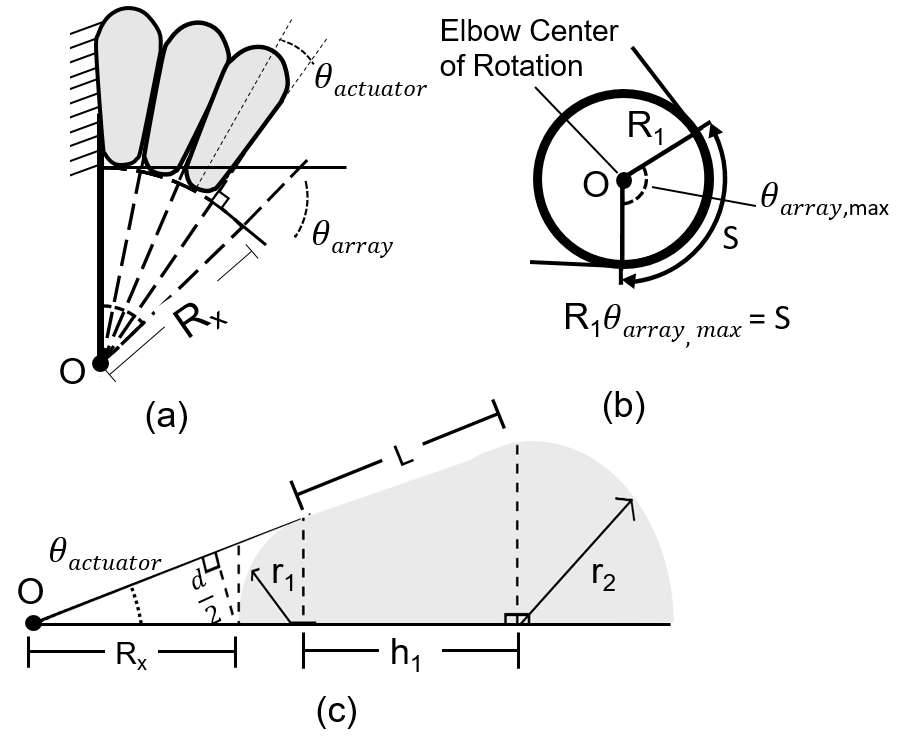
\includegraphics[width=0.45\textwidth]{model3.PNG}
% \caption{(a) Simple bladder arrangement demonstrating interactions in the array.  (b) Spherical elbow joint representation of constant radius. $S$. The length of the actuator array is defined with this model. (c) Section view of an individual actuator depicting dimensions used in calculating the interacting area. }
% \label{fig:hotness}
% \end{figure}
%\textcolor{red}{S=R1theta0 and theta1 is centerline to interacting edge }



% \begin{equation}\label{r1}
% 	r_1(\theta_{actuator})  = \frac{d}{2cos(\theta_{actuator})}.
% \end{equation}

% While the major radius, $r_2$, also utilizes the tangent, the solution is expressed as
%  \begin{equation}\label{r2}
% 	r_2(\theta_{actuator})  = -b + \sqrt{\frac{b^2-4ac}{2a}} ,
% \end{equation}
% where $a$, $b$, and $c$ are defined by

% \begin{equation}\label{a}
% 	a = 1+\frac{1}{(\pi R+\sqrt{(R_x+r_1)^2+r_1^2})^2}+(\frac{\pi}{2})^2 ,
% \end{equation}
% \begin{equation}\label{a}
% 	b = \pi^2R+\pi\sqrt{(R_x+r_1)^2+r_1^2}-\frac{\pi^2r_1}{2} ,
% \end{equation}
% \begin{equation}\label{a}
% \begin{aligned}
% \begin{multlined}
% 	c = (\pi R+\sqrt{(R_x+r_1)^2+r_1^2})^2- (\pi R+\lambda)^2...\\\\
%    +\pi^2Rr_1-(\frac{\pi R}{2})^2+\sqrt{(R_x+r_q)^2+r_1^2}\pi r_1 .
%     \end{multlined}
%     \end{aligned}
% \end{equation}



\section{Conclusion and Future Work}

In this paper, the design, development, and evaluation of a novel, user-mounted, fabric Soft Poly-Limb (fSPL) is introduced. The highly-articulated, soft fSPL is designed towards supporting and assisting impaired individuals, for example CSM patients, with daily living tasks. The fSPL’s geometrical parameters are initially optimized and experimentally validated using quasi-static computational FEM models providing design guidelines for the community to design an fSPL based on the desired payload against gravity and bending ability.

We demonstrated that this successful implementation of the fSPL can carry up to 1.5$kg$ while still being able to maneuver in space with various pick-and-place experiments, meeting the requirements of dealing with daily objects and tasks. Each fSPL segment, the f3CBA, is able to effectively lift 6.3$kg$, up to its 17 times its own weight without any effects of torsion noticed. By employing the whole body grasping strategy, the fSPL can wrap and carry load of up to 4.5$kg$, up to 4 times it’s own body weight of 1.11$kg$.

The fSPL was shown to be capable of safely working around a user with a large workspace and be able to safely interact with the environment. The fSPL’s segmented modular design allows the rapid swapping of actuators from the bladder array pouches for maintenance as well as interchangeable and replaceable segments. The end-effector of the fSPL is also modifiable to different types of graspers aside from the suction cup.

Future work will introduce the exploration of multi-mounting positions and multi-interacting fSPLs on one user to expand the user’s workspace and capabilities of controlling multi-external limbs. In this work, the fSPL was controlled using a joystick module but various user-detection methods have been tested in our previous work, as well was sEMG for a hands-free method of controlling the limb \cite{Nguyen2018}. Further efforts are being made to improve and explore other hands-free, user-intent detection for external robotic limbs.

Another limitation of the fSPL is the tethering of the system. We plan to look at decentralized and distributed on-board actuation and power supply systems that are capable of controlling such a complicated system. Future efforts are being made to control the SPL using distributed sensing and control methods \cite{Wenlong2018} with the exploration of soft-distributed and embedded sensing technologies as well. 

In total, we believe that this work provides the readers with the capability of designing highly lightweight and soft robotic limbs capable of being easily stored and deployed on-site capable of support the versatile amount of activities of daily living.




%%%%%%%%%%%%%%%%%%%%%%%%%%%%%%%%%%%%%%%%%%%%%%%%%%%%%%%%%%%%%%%%%%%%%%%%%%%%%%%%

\section*{ACKNOWLEDGMENTS} 
This work was supported in part by the National Science Foundation under Grant CMMI-1800940.

%%%%%%%%%%%%%%%%%%%%%%%%%%%%%%%%%%%%%%%%%%%%%%%%%%%%%%%%%%%%%%%%%%%%%%%%%%%%%%%%



%%%%%%%%%%%%%%%%%%%%%%%%%%%%%%%%%%%%%%%%%%%%%%%%%%%%%%%%%%%%%%%%%%%%%%%%%%%%%%%%
%%%%%%%%%%%%%%%%%%%%%%%%%%%%%%%%%%%%%%%%%%%%%%%%%%%%%%%%%%%%%%%%%%%%%%%%%%%%%%%%


% ********************************** Bibliography ******************************
\bibliographystyle{unsrt}
%\bibliographystyle{plain}
%\bibliographystyle{plainnat} % use this to have URLs listed in References
%\cleardoublepage
\bibliography{ICRA2019.bib} % Path to your References.bib file



% \begin{thebibliography}{99}
% \bibitem{c1} G. O. Young, ÒSynthetic structure of industrial plastics (Book style with paper title and editor),Ó 	in Plastics, 2nd ed. vol. 3, J. Peters, Ed.  New York: McGraw-Hill, 1964, pp. 15Ð64.
% \bibitem{c2} W.-K. Chen, Linear Networks and Systems (Book style).	Belmont, CA: Wadsworth, 1993, pp. 123Ð135.
% \bibitem{c3} H. Poor, An Introduction to Signal Detection and Estimation.   New York: Springer-Verlag, 1985, ch. 4.
% \bibitem{c4} B. Smith, ÒAn approach to graphs of linear forms (Unpublished work style),Ó unpublished.
% \bibitem{c5} E. H. Miller, ÒA note on reflector arrays (Periodical styleÑAccepted for publication),Ó IEEE Trans. Antennas Propagat., to be publised.
% \bibitem{c6} J. Wang, ÒFundamentals of erbium-doped fiber amplifiers arrays (Periodical styleÑSubmitted for publication),Ó IEEE J. Quantum Electron., submitted for publication.
% \bibitem{c7} C. J. Kaufman, Rocky Mountain Research Lab., Boulder, CO, private communication, May 1995.
% \bibitem{c8} Y. Yorozu, M. Hirano, K. Oka, and Y. Tagawa, ÒElectron spectroscopy studies on magneto-optical media and plastic substrate interfaces(Translation Journals style),Ó IEEE Transl. J. Magn.Jpn., vol. 2, Aug. 1987, pp. 740Ð741 [Dig. 9th Annu. Conf. Magnetics Japan, 1982, p. 301].
% \bibitem{c9} M. Young, The Techincal Writers Handbook.  Mill Valley, CA: University Science, 1989.
% \bibitem{c10} J. U. Duncombe, ÒInfrared navigationÑPart I: An assessment of feasibility (Periodical style),Ó IEEE Trans. Electron Devices, vol. ED-11, pp. 34Ð39, Jan. 1959.
% \bibitem{c11} S. Chen, B. Mulgrew, and P. M. Grant, ÒA clustering technique for digital communications channel equalization using radial basis function networks,Ó IEEE Trans. Neural Networks, vol. 4, pp. 570Ð578, July 1993.
% \bibitem{c12} R. W. Lucky, ÒAutomatic equalization for digital communication,Ó Bell Syst. Tech. J., vol. 44, no. 4, pp. 547Ð588, Apr. 1965.
% \bibitem{c13} S. P. Bingulac, ÒOn the compatibility of adaptive controllers (Published Conference Proceedings style),Ó in Proc. 4th Annu. Allerton Conf. Circuits and Systems Theory, New York, 1994, pp. 8Ð16.
% \bibitem{c14} G. R. Faulhaber, ÒDesign of service systems with priority reservation,Ó in Conf. Rec. 1995 IEEE Int. Conf. Communications, pp. 3Ð8.
% \bibitem{c15} W. D. Doyle, ÒMagnetization reversal in films with biaxial anisotropy,Ó in 1987 Proc. INTERMAG Conf., pp. 2.2-1Ð2.2-6.
% \bibitem{c16} G. W. Juette and L. E. Zeffanella, ÒRadio noise currents n short sections on bundle conductors (Presented Conference Paper style),Ó presented at the IEEE Summer power Meeting, Dallas, TX, June 22Ð27, 1990, Paper 90 SM 690-0 PWRS.
% \bibitem{c17} J. G. Kreifeldt, ÒAn analysis of surface-detected EMG as an amplitude-modulated noise,Ó presented at the 1989 Int. Conf. Medicine and Biological Engineering, Chicago, IL.
% \bibitem{c18} J. Williams, ÒNarrow-band analyzer (Thesis or Dissertation style),Ó Ph.D. dissertation, Dept. Elect. Eng., Harvard Univ., Cambridge, MA, 1993. 
% \bibitem{c19} N. Kawasaki, ÒParametric study of thermal and chemical nonequilibrium nozzle flow,Ó M.S. thesis, Dept. Electron. Eng., Osaka Univ., Osaka, Japan, 1993.
% \bibitem{c20} J. P. Wilkinson, ÒNonlinear resonant circuit devices (Patent style),Ó U.S. Patent 3 624 12, July 16, 1990.
% \end{thebibliography}




\end{document}
